% A LaTeX template for MSc Thesis submissions to 
% Politecnico di Milano (PoliMi) - School of Industrial and Information Engineering
%
% https://www.ingindinf.polimi.it/it/didattica/lezioni-e-esami/esami-di-laurea-e-laurea-magistrale
%
% S. Bonetti, A. Gruttadauria, G. Mescolini, A. Zingaro
% e-mail: template-tesi-ingind@polimi.it
%
% Last Revision: October 2021
%
% Copyright 2021 Politecnico di Milano, Italy. NC-BY

\documentclass{Configuration_Files/PoliMi3i_thesis}

%------------------------------------------------------------------------------
%	REQUIRED PACKAGES AND  CONFIGURATIONS
%------------------------------------------------------------------------------

% CONFIGURATIONS
\usepackage{parskip} % For paragraph layout
\usepackage{setspace} % For using single or double spacing
\usepackage{emptypage} % To insert empty pages
\usepackage{multicol} % To write in multiple columns (executive summary)
\setlength\columnsep{15pt} % Column separation in executive summary
\setlength\parindent{0pt} % Indentation
\raggedbottom  

% PACKAGES FOR TITLES
\usepackage{titlesec}
% \titlespacing{\section}{left spacing}{before spacing}{after spacing}
\titlespacing{\section}{0pt}{3.3ex}{2ex}
\titlespacing{\subsection}{0pt}{3.3ex}{1.65ex}
\titlespacing{\subsubsection}{0pt}{3.3ex}{1ex}
\usepackage{color}

% PACKAGES FOR LANGUAGE AND FONT
\usepackage[english]{babel} % The document is in English  
\usepackage[utf8]{inputenc} % UTF8 encoding
\usepackage[T1]{fontenc} % Font encoding
\usepackage[11pt]{moresize} % Big fonts

% PACKAGES FOR IMAGES
\usepackage{graphicx}
\usepackage{transparent} % Enables transparent images
\usepackage{eso-pic} % For the background picture on the title page
\usepackage{subfig} % Numbered and caption subfigures using \subfloat.
\usepackage{tikz} % A package for high-quality hand-made figures.
\usetikzlibrary{}
\graphicspath{{./Images/}} % Directory of the images
\usepackage{caption} % Coloured captions
\usepackage{xcolor} % Coloured captions
\usepackage{amsthm,thmtools,xcolor} % Coloured "Theorem"
\usepackage{float}

% STANDARD MATH PACKAGES
\usepackage{amsmath}
\usepackage{amsthm}
\usepackage{amssymb}
\usepackage{amsfonts}
\usepackage{bm}
\usepackage[overload]{empheq} % For braced-style systems of equations.
\usepackage{fix-cm} % To override original LaTeX restrictions on sizes

% PACKAGES FOR TABLES
\usepackage{tabularx}
\usepackage{longtable} % Tables that can span several pages
\usepackage{ltablex} % Tables that can span several page and have automatic width
\usepackage{colortbl}

% PACKAGES FOR ALGORITHMS (PSEUDO-CODE)
\usepackage{algorithm}
\usepackage{algorithmic}

% PACKAGES FOR REFERENCES & BIBLIOGRAPHY
\usepackage[colorlinks=true,linkcolor=black,anchorcolor=black,citecolor=black,filecolor=black,menucolor=black,runcolor=black,urlcolor=black]{hyperref} % Adds clickable links at references
\usepackage{cleveref}
\usepackage[square, numbers, sort&compress]{natbib} % Square brackets, citing references with numbers, citations sorted by appearance in the text and compressed
\bibliographystyle{abbrvnat} % You may use a different style adapted to your field

% OTHER PACKAGES
\usepackage{pdfpages} % To include a pdf file
\usepackage{afterpage}
\usepackage{lipsum} % DUMMY PACKAGE
\usepackage{fancyhdr} % For the headers
\fancyhf{}

% Input of configuration file. Do not change config.tex file unless you really know what you are doing. 
% Set the geometric layout of the document
\usepackage{geometry}
\geometry{
  top=2.8cm,
  left = 1.9cm,
  right = 1.9cm,
  bottom=2.0cm,
  headheight= 2cm,
  headsep= 0cm,
}
\raggedbottom 

% Create color bluePoli (-> manuale grafica coordinata:  https://www.polimi.it/fileadmin/user_upload/il_Politecnico/grafica-coordinata/2015_05_11_46xy_manuale_grafica_coordinata.pdf)
\definecolor{bluePoli}{cmyk}{0.4,0.1,0,0.4}

% Custom theorem environments
\declaretheoremstyle[
  headfont=\color{bluePoli}\normalfont\bfseries,
  bodyfont=\color{black}\normalfont\itshape,
]{colored}

\captionsetup[figure]{labelfont={color=bluePoli}} % Set colour of the captions
\captionsetup[table]{labelfont={color=bluePoli}} % Set colour of the captions
\captionsetup[algorithm]{labelfont={color=bluePoli}} % Set colour of the captions

\theoremstyle{colored}
\newtheorem{theorem}{Theorem}[section]
\newtheorem{proposition}{Proposition}[section]

% Enhances the features of the standard "table" and "tabular" environments.
\newcommand\T{\rule{0pt}{2.6ex}}
\newcommand\B{\rule[-1.2ex]{0pt}{0pt}}

% Algorithm description
\newcounter{algsubstate}
\renewcommand{\thealgsubstate}{\alph{algsubstate}}
\newenvironment{algsubstates}{
    \setcounter{algsubstate}{0}%
    \renewcommand{\STATE}{%
    \stepcounter{algsubstate}%
    \Statex {\small\thealgsubstate:}\space}
    }{}
    
% Custom theorem environment
\newcolumntype{L}[1]{>{\raggedright\let\newline\\\arraybackslash\hspace{0pt}}m{#1}}
\newcolumntype{C}[1]{>{\centering\let\newline\\\arraybackslash\hspace{0pt}}m{#1}}
\newcolumntype{R}[1]{>{\raggedleft\let\newline\\\arraybackslash\hspace{0pt}}m{#1}}

% Custom itemize environment
\setlist[itemize,1]{label=$\bullet$}
\setlist[itemize,2]{label=$\circ$}
\setlist[itemize,3]{label=$-$}
\setlist{nosep}

% Set separation of columns 
\setlength{\columnsep}{30pt}

% Create command for background pic
\newcommand\BackgroundPic{% Adding background picture
	\put(237,365){
		\parbox[b][\paperheight]{\paperwidth}{%
			\vfill
			\centering
			\transparent{0.4}
			
\includegraphics[width=0.44\paperwidth]{raggiera_polimi.eps}%
			\vfill
}}}

% Set indentation
\setlength\parindent{0pt}

% Custom title commands
\titleformat{\section}
{\color{bluePoli}\normalfont\Large\bfseries}
{\color{bluePoli}\thesection.}{1em}{}
\titlespacing*{\section}
{0pt}{2ex}{1ex}

\titleformat{\subsection}
{\color{bluePoli}\normalfont\large\bfseries}
{\color{bluePoli}\thesubsection.}{1em}{}
\titlespacing*{\subsection}
{0pt}{2ex}{1ex}

% Custom headers and footers
\pagestyle{fancy}
\fancyhf{}
      
\fancyfoot{}
\fancyfoot[C]{\thepage} % page
\renewcommand{\headrulewidth}{0mm} % headrule width
\renewcommand{\footrulewidth}{0mm} % footrule width

\makeatletter
\patchcmd{\headrule}{\hrule}{\color{black}\hrule}{}{} % headrule
\patchcmd{\footrule}{\hrule}{\color{black}\hrule}{}{} % footrule
\makeatother

% -> Create the header
\chead[C]{
\centering
\begin{tcolorbox}[arc=0pt, boxrule=0pt, colback=bluePoli!60, width=\textwidth, colupper=white, top=1.7mm, bottom=1.7mm]
    \textbf{Executive summary} \hfill \textbf{\author}  
\end{tcolorbox}
}

%----------------------------------------------------------------------------
%	NEW COMMANDS DEFINED
%----------------------------------------------------------------------------

% EXAMPLES OF NEW COMMANDS
\newcommand{\bea}{\begin{eqnarray}} % Shortcut for equation arrays
\newcommand{\eea}{\end{eqnarray}}
\newcommand{\e}[1]{\times 10^{#1}}  % Powers of 10 notation

%----------------------------------------------------------------------------
%	ADD YOUR PACKAGES (be careful of package interaction)
%----------------------------------------------------------------------------

\usepackage{array,tabularx}
\usepackage{longtable}
\usepackage{multirow}
\usepackage{svg}
\usepackage[utf8]{inputenc}
\usepackage{xcolor}
\usepackage{graphicx,wrapfig} % For figures inside the text
\usepackage{listings} % Show code in text
\usepackage{mdframed} % Example box \begin{example} ... \end{example}

%----------------------------------------------------------------------------
%	ADD YOUR DEFINITIONS AND COMMANDS (be careful of existing commands)
%----------------------------------------------------------------------------

% Better inline code
\definecolor{light-gray}{gray}{0.95}
\newcommand{\inlinecode}[1]{\colorbox{light-gray}{\texttt{#1}}}

% Show code in text (JSON)
\colorlet{punct}{red!60!black}
\definecolor{CodeBackground}{HTML}{EEEEEE}
\definecolor{delim}{RGB}{20,105,176}
\colorlet{numb}{magenta!60!black}
\lstdefinelanguage{json}{
    basicstyle=\normalfont\ttfamily,
    numbers=left,
    numberstyle=\scriptsize,
    stepnumber=1,
    numbersep=8pt,
    showstringspaces=false,
    breaklines=true,
    frame=lines,
    backgroundcolor=\color{CodeBackground},
    literate=
     *{:}{{{\color{punct}{:}}}}{1}
      {,}{{{\color{punct}{,}}}}{1}
      {\{}{{{\color{delim}{\{}}}}{1}
      {\}}{{{\color{delim}{\}}}}}{1}
      {[}{{{\color{delim}{[}}}}{1}
      {]}{{{\color{delim}{]}}}}{1},
}

% Show code in text (JavaScript)
\definecolor{lightgray}{rgb}{.9,.9,.9}
\definecolor{darkgray}{rgb}{.4,.4,.4}
\definecolor{purple}{rgb}{0.65, 0.12, 0.82}
\lstdefinelanguage{javascript}{
  keywords={typeof, new, true, false, catch, function, return, null, catch, switch, var, if, in, while, do, else, case, break},
  keywordstyle=\color{blue}\bfseries,
  ndkeywords={const, await, class, export, boolean, throw, implements, import, this},
  ndkeywordstyle=\color{darkgray}\bfseries,
  identifierstyle=\color{black},
  sensitive=false,
  comment=[l]{//},
  morecomment=[s]{/*}{*/},
  commentstyle=\color{purple}\ttfamily,
  stringstyle=\color{red}\ttfamily,
  morestring=[b]',
  morestring=[b]"
}
\lstset{
   language=javascript,
   backgroundcolor=\color{lightgray},
   extendedchars=true,
   basicstyle=\footnotesize\ttfamily,
   showstringspaces=false,
   showspaces=false,
   %numbers=right,
   %numberstyle=\footnotesize,
   %numbersep=8pt,
   tabsize=2,
   breaklines=true,
   showtabs=false,
   captionpos=b
}

% Show code in text (BASH)
\lstdefinelanguage{bash}{
    basicstyle=\normalfont\ttfamily,
    numbers=left,
    numberstyle=\scriptsize,
    stepnumber=1,
    numbersep=8pt,
    showstringspaces=false,
    breaklines=true,
    frame=lines,
    backgroundcolor=\color{CodeBackground},
}

% Show code in text (YAML)
\newcommand\YAMLcolonstyle{\color{red}\mdseries}
\newcommand\YAMLkeystyle{\color{black}\bfseries}
\newcommand\YAMLvaluestyle{\color{blue}\mdseries}
\makeatletter
\newcommand\language@yaml{yaml} % macro expanding to the name of the language (handy if you decide to change it further down the road)
\expandafter\expandafter\expandafter\lstdefinelanguage
\expandafter{\language@yaml}
{
    keywords={true,false,null,y,n},
    keywordstyle=\color{darkgray}\bfseries,
    backgroundcolor=\color{CodeBackground},
    basicstyle=\YAMLkeystyle, % assuming a key comes first
    numbers=left,
    numberstyle=\scriptsize,
    stepnumber=1,
    numbersep=8pt,
    sensitive=false,
    comment=[l]{\#},
    morecomment=[s]{/*}{*/},
    commentstyle=\color{purple}\ttfamily,
    stringstyle=\YAMLvaluestyle\ttfamily,
    moredelim=[l][\color{orange}]{\&},
    moredelim=[l][\color{magenta}]{*},
    moredelim=**[il][\YAMLcolonstyle{:}\YAMLvaluestyle]{:}, % switch to value style at :
    morestring=[b]',
    morestring=[b]",
    literate =  {---}{{\ProcessThreeDashes}}3
                {>}{{\textcolor{red}\textgreater}}1     
                {|}{{\textcolor{red}\textbar}}1 
                {\ -\ }{{\mdseries\ -\ }}3,
}
\lst@AddToHook{EveryLine}{\ifx\lst@language\language@yaml\YAMLkeystyle\fi} % switch to key style at EOL
\makeatother
\newcommand\ProcessThreeDashes{\llap{\color{cyan}\mdseries-{-}-}}

% Example box. \begin{example} ... \end{example}
\definecolor{ExampleBoxBackground}{HTML}{999999}
\newmdenv[ % Define mdframe settings and store as leftrule
  linecolor=ExampleBoxBackground,
  linewidth = 2pt,
  topline=false,
  bottomline=false,
  rightline=false,
  skipabove=\topsep,
  skipbelow=\topsep
]{leftrule}
\newenvironment{example}{
	\medskip
	\begin{leftrule}
	\textbf{Example}
	\medskip
	\color{black!60}
   	\newline%
}{
	\medskip
    \end{leftrule}
}

%----------------------------------------------------------------------------
%	BEGIN OF YOUR DOCUMENT
%----------------------------------------------------------------------------

\begin{document}

\fancypagestyle{plain}{%
\fancyhf{} % Clear all header and footer fields
\fancyhead[RO,RE]{\thepage} %RO=right odd, RE=right even
\renewcommand{\headrulewidth}{0pt}
\renewcommand{\footrulewidth}{0pt}}

%----------------------------------------------------------------------------
%	TITLE PAGE
%----------------------------------------------------------------------------

\pagestyle{empty} % No page numbers
\frontmatter % Use roman page numbering style (i, ii, iii, iv...) for the preamble pages

\puttitle{
	title=Location-Aware and Stateful Serverless Computing on the Edge, % Title of the thesis
	name=Dennis Motta, % Author Name and Surname
	course=Computer Science and Engineering, % Study Programme
	ID  = 940064,  % Student ID number (numero di matricola)
	advisor= Alessandro Margara, % Supervisor name
	coadvisor={Gianpaolo Cugola}, % Co-Supervisor name, remove this line if there is none
	academicyear={2020-2021},  % Academic Year
} % These info will be put into your Title page 

%----------------------------------------------------------------------------
%	PREAMBLE PAGES: ABSTRACT (inglese e italiano), EXECUTIVE SUMMARY
%----------------------------------------------------------------------------
\startpreamble
\setcounter{page}{1} % Set page counter to 1

% ABSTRACT IN ENGLISH
\chapter*{Abstract}

The popularity and proliferation of smart devices (e.g., smartphones, wearable devices, Internet-of-Things sensors) is resulting in an unprecedented growth in the amount of collected data. The current most popular approaches to manage this huge amount of data typically rely on cloud platforms located at the core of the infrastructure.

As the number of devices and the amount of data they generate increases, such core-centric approaches are becoming increasingly inefficient as they need to transfer data back and forth between the core and the devices. Furthermore, the latencies associated with such data transfer are affected by the huge travel-distance needed to make the device communicate to the central cloud platform.

To deal with the aforementioned situation new approaches have been introduced in both academia and industry, exploiting the power of the edge of the network to perform the computation closer to the data source. We noticed a discrepancy between the approaches proposed in research and in industry: research frequently assumes the possibility of running virtual machines or long-running containers on the edge. However, most real-world web infrastructure companies do not comply with this assumption due to the limited resource available in the edge.

In this thesis we study the state of the art for stateful computations and data processing on the edge and after carefully analyzing the issues and the needs of the scenario we show the use cases predominantly affected by bandwidth and latency constraints. We then show the current frameworks available in the industry and notice how these solutions do not cover the use cases found. So we then propose a serverless approach effectively applicable by web infrastructure companies, that takes into consideration the problem of the scarcity of the resources while still allowing quite powerful stateful computations on the edge. We also show how we implemented this new approach through a working prototype, and finally we investigate the gains developers may obtain by using our approach. We demonstrate how several use cases can benefit from this new system through discrete-event simulation, since running our prototype on an emulation of a global edge network was infeasible due to the sheer amount of resources needed to emulate even a small edge network.

\textbf{Keywords:} Edge Computing, Serverless, FaaS, Stateful



\iffalse
\chapter*{Abstract} 
Here goes the Abstract in English of your thesis followed by a list of keywords.
The Abstract is a concise summary of the content of the thesis (single page of text)
and a guide to the most important contributions included in your thesis.
The Abstract is the very last thing you write.
It should be a self-contained text and should be clear to someone who hasn't (yet) read the whole manuscript.
The Abstract should contain the answers to the main scientific questions that have been addressed in your thesis.
It needs to summarize the adopted motivations and the adopted methodological approach as well as the findings of your work and their relevance and impact.
The Abstract is the part appearing in the record of your thesis inside POLITesi,
the Digital Archive of PhD and Master Theses (Laurea Magistrale) of Politecnico di Milano.
The Abstract will be followed by a list of four to six keywords.
Keywords are a tool to help indexers and search engines to find relevant documents.
To be relevant and effective, keywords must be chosen carefully.
They should represent the content of your work and be specific to your field or sub-field.
Keywords may be a single word or two to four words. 
\\
\\
\textbf{Keywords:} here, the keywords, of your thesis % Keywords
\fi


% ABSTRACT IN ITALIAN
\chapter*{Sommario}

La popolarità e la proliferazione di dispositivi intelligenti (e.g., smartphone, dispositivi indossabili, sensori Internet-of-Things) sta determinando una crescita senza precedenti della quantità di dati raccolti. Gli approcci attualmente più diffusi per gestire questa enorme quantità di dati si basano in genere su piattaforme cloud situate al centro dell'infrastruttura.

Con l'aumento del numero di dispositivi e della quantità di dati generati, tali approcci basati su un core centrale stanno diventando sempre più inefficienti poiché devono trasferire i dati avanti e indietro tra il core e i dispositivi. Inoltre, le latenze associate a tale trasferimento di dati sono influenzate dall'enorme distanza di viaggio necessaria per far comunicare il dispositivo con la piattaforma cloud centrale.

Per affrontare la situazione sono stati introdotti nuovi approcci sia nel mondo accademico che nell'industria, sfruttando la potenza dell'edge della rete per eseguire il calcolo più vicino alla fonte dei dati. Abbiamo notato una discrepanza tra gli approcci proposti nella ricerca e nell'industria: la ricerca presuppone spesso la possibilità di eseguire macchine virtuali o container di lunga durata sull'edge. Tuttavia, la maggior parte delle aziende di infrastruttura web non rispettano questa ipotesi a causa delle risorse limitate disponibili nell'edge.

In questa tesi studiamo lo stato dell'arte per le computazioni con stato e per l'elaborazione dei dati sull'edge, e dopo aver analizzato attentamente le problematiche e le esigenze dello scenario mostriamo i casi d'uso prevalentemente affetti da vincoli di larghezza di banda e latenza. Mostriamo quindi i framework attuali disponibili nel settore e notiamo come queste soluzioni non coprono i casi d'uso trovati. Quindi proponiamo un approccio serverless effettivamente applicabile dalle aziende di infrastrutture web, che tenga conto del problema della scarsità delle risorse pur consentendo computazioni stateful abbastanza potenti sull'edge. Mostriamo anche come abbiamo implementato questo nuovo approccio attraverso un prototipo funzionante, e infine esaminiamo i benefici che gli sviluppatori possono ottenere usando il nostro approccio. Dimostriamo come diversi casi d'uso possono trarre vantaggio da questo nuovo sistema attraverso la simulazione a eventi discreti, poiché l'esecuzione del nostro prototipo su un'emulazione di una rete edge globale era impossibile a causa dell'enorme quantità di risorse necessarie per emulare anche una piccola rete edge.

\textbf{Keywords:} Edge Computing, Serverless, FaaS, Stateful


% ACKNOWLEDGEMENTS
\chapter{Acknowledgements}
In this chapter, you can acknowledge the people that were somehow helpful in the realization of the thesis. It is better to keep this chapter formal, you can add the friendly thanks at the end (chapter Thanks).

%----------------------------------------------------------------------------
%	LIST OF CONTENTS/FIGURES/TABLES/SYMBOLS
%---------------------------------------------------------------------------

% TABLE OF CONTENTS
\thispagestyle{empty}
\tableofcontents % Table of contents 
\thispagestyle{empty}
\cleardoublepage


% LIST OF FIGURES
\listoffigures

% LIST OF TABLES
\listoftables

% LIST OF SYMBOLS
\chapter*{List of Acronyms and Abbrevations}
\begin{table}[H]
\begin{tabular}{p{2cm}l}
API    & Application Programming Interface                         \\[5pt]
BGP    & Border Gateway Protocol                                   \\[5pt]
CDN    & Content Delivery Network                                  \\[5pt]
CLI    & Command Line Interface                                    \\[5pt]
FaaS   & Function-as-a-Service                                     \\[5pt]
GB     & Gigabyte                                                  \\[5pt]
GPS    & Global Positioning System                                 \\[5pt]
HTTP   & HyperText Transfer Protocol                               \\[5pt]
ICFEC  & IEEE International Conference on Fog and Edge Computing   \\[5pt]
ID     & Identifier                                                \\[5pt]
IDE    & Integrated Development Environment                        \\[5pt]
IP     & Internet Protocol                                         \\[5pt]
IoT    & Internet-of-Things                                        \\[5pt]
JSON   & JavaScript Object Notation                                \\[5pt]
KB     & Kilobyte                                                  \\[5pt]
MB     & Megabyte                                                  \\[5pt]
OS     & Operating System                                          \\[5pt]
RAM    & Random Access Memory                                      \\[5pt]
RQ     & Research Questions                                        \\[5pt]
UI     & User interface                                            \\[5pt]
URL    & Uniform Resource Locator                                  \\[5pt]
VM     & Virtual Machine                                           \\[5pt]
\end{tabular}
\end{table}


%-------------------------------------------------------------------------
%	THESIS MAIN TEXT
%-------------------------------------------------------------------------
% In the main text of your thesis you can write the chapters in two different ways:
%
%(1) As presented in this template you can write:
%    \chapter{Title of the chapter}
%    *body of the chapter*
%
%(2) You can write your chapter in a separated .tex file and then include it in the main file with the following command:
%    \chapter{Title of the chapter}
%    \input{chapter_file.tex}
%
% Especially for long thesis, we recommend you the second option.

\addtocontents{toc}{\vspace{2em}} % Add a gap in the Contents, for aesthetics
\mainmatter % Begin numeric (1,2,3...) page numbering

% --------------------------------------------------------------------------
% NUMBERED CHAPTERS % Regular chapters following
% --------------------------------------------------------------------------
%\chapter{Chapter one}
\label{ch:chapter_one}%
% The \label{...}% enables to remove the small indentation that is generated, always leave the % symbol.

In this chapter additional useful information are reported.

\section{Sections and subsections}
\label{sec:section_name}
Chapters are typically subdivided into sections and subsections, and, optionally,
subsubsections, paragraphs and subparagraphs.
All can have a title, but only sections and subsections are numbered.
A new section is created by the command
\begin{verbatim}
\section{Title of the section}
\end{verbatim}
The numbering can be turned off by using \verb|\section*{}|.
\\
A new subsection is created by the command
\begin{verbatim}
\subsection{Title of the subsection}
\end{verbatim}
and, similarly, the numbering can be turned off by adding an asterisk as follows 
\begin{verbatim}
\subsection*{}
\end{verbatim}

\section{Equations}
\label{sec:eqs}
This section gives some examples of writing mathematical equations in your thesis.

Maxwell's equations read:
\begin{subequations}
    \label{eq:maxwell}
    \begin{align}[left=\empheqlbrace]
    \nabla\cdot \bm{D} & = \rho, \label{eq:maxwell1} \\
    \nabla \times \bm{E} +  \frac{\partial \bm{B}}{\partial t} & = \bm{0}, \label{eq:maxwell2} \\
    \nabla\cdot \bm{B} & = 0, \label{eq:maxwell3} \\
    \nabla \times \bm{H} - \frac{\partial \bm{D}}{\partial t} &= \bm{J}. \label{eq:maxwell4}
    \end{align}
\end{subequations}

Equation~\eqref{eq:maxwell} is automatically labeled by \texttt{cleveref},
as well as Equation~\eqref{eq:maxwell1} and Equation~\eqref{eq:maxwell3}.
Thanks to the \verb|cleveref| package, there is no need to use \verb|\eqref|.
Remember that Equations have to be numbered only if they are referenced in the text.

Equations~\eqref{eq:maxwell_multilabels1}, \eqref{eq:maxwell_multilabels2}, \eqref{eq:maxwell_multilabels3}, and \eqref{eq:maxwell_multilabels4} show again Maxwell's equations without brace:
\begin{align}
    \nabla\cdot \bm{D} & = \rho, \label{eq:maxwell_multilabels1} \\
    \nabla \times \bm{E} +  \frac{\partial \bm{B}}{\partial t} &= \bm{0}, \label{eq:maxwell_multilabels2} \\
    \nabla\cdot \bm{B} & = 0, \label{eq:maxwell_multilabels3} \\
    \nabla \times \bm{H} - \frac{\partial \bm{D}}{\partial t} &= \bm{J} \label{eq:maxwell_multilabels4}.
\end{align}

Equation~\eqref{eq:maxwell_singlelabel} is the same as before,
but with just one label:
\begin{equation}
    \label{eq:maxwell_singlelabel}
    \left\{
    \begin{aligned}
    \nabla\cdot \bm{D} & = \rho, \\
    \nabla \times \bm{E} +  \frac{\partial \bm{B}}{\partial t} &= \bm{0},\\
    \nabla\cdot \bm{B} & = 0, \\
    \nabla \times \bm{H} - \frac{\partial \bm{D}}{\partial t} &= \bm{J}.
    \end{aligned}
    \right.
\end{equation}

\section{Figures, Tables and Algorithms}
Figures, Tables and Algorithms have to contain a Caption that describe their content, and have to be properly reffered in the text.

\subsection{Figures}
\label{subsec:figures}

For including pictures in your text you can use \texttt{TikZ} for high-quality hand-made figures,
or just include them as usual with the command
\begin{verbatim}
\includegraphics[options]{filename.xxx}
\end{verbatim}
Here xxx is the correct format, e.g. \verb|.png|, \verb|.jpg|, \verb|.eps|, \dots.

\begin{figure}[H]
    \centering
    
\includegraphics[width=0.3\textwidth]{logo_polimi_scritta.eps}
    \caption{Caption of the Figure to appear in the List of Figures.}
    \label{fig:quadtree}
\end{figure}

Thanks to the \texttt{\textbackslash subfloat} command, a single figure, such as Figure~\ref{fig:quadtree},
can contain multiple sub-figures with their own caption and label, e.g. \color{black} Figure~\ref{fig:polimi_logo1} and Figure~\ref{fig:polimi_logo2}. 

\begin{figure}[H]
    \centering
    \subfloat[One PoliMi logo.\label{fig:polimi_logo1}]{
        
\includegraphics[scale=0.5]{Images/logo_polimi_scritta.eps}
    }
    \quad
    \subfloat[Another one PoliMi logo.\label{fig:polimi_logo2}]{
        
\includegraphics[scale=0.5]{Images/logo_polimi_scritta2.eps}
    }
    \caption[Shorter caption]{This is a very long caption you don't want to appear in the List of Figures.}
    \label{fig:quadtree2}
\end{figure}


\subsection{Tables}
\label{subsec:tables}

Within the environments \texttt{table} and  \texttt{tabular} you can create very fancy tables as the one shown in Table~\ref{table:example}.
\begin{table}[H]
    \caption*{\textbf{Title of Table (optional)}}
    \centering 
    \begin{tabular}{|p{3em} c c c |}
    \hline
    \rowcolor{bluepoli!40} % comment this line to remove the color
     & \textbf{column 1} & \textbf{column 2} & \textbf{column 3} \T\B \\
    \hline \hline
    \textbf{row 1} & 1 & 2 & 3 \T\B \\
    \textbf{row 2} & $\alpha$ & $\beta$ & $\gamma$ \T\B\\
    \textbf{row 3} & alpha & beta & gamma \B\\
    \hline
    \end{tabular}
    \\[10pt]
    \caption{Caption of the Table to appear in the List of Tables.}
    \label{table:example}
\end{table}

You can also consider to highlight selected columns or rows in order to make tables more readable.
Moreover, with the use of \texttt{table*} and the option \texttt{bp} it is possible to align them at the bottom of the page. One example is presented in Table~\ref{table:exampleC}. 

\begin{table}[H]
\centering 
    \begin{tabular}{|p{3em} | c | c | c | c | c | c|}
    \hline
%    \rowcolor{bluepoli!40}
     & \textbf{column1} & \textbf{column2} & \textbf{column3} & \textbf{column4} & \textbf{column5} & \textbf{column6} \T\B \\
    \hline \hline
    \textbf{row1} & 1 & 2 & 3 & 4 & 5 & 6 \T\B\\
    \textbf{row2} & a & b & c & d & e & f \T\B\\
    \textbf{row3} & $\alpha$ & $\beta$ & $\gamma$ & $\delta$ & $\phi$ & $\omega$ \T\B\\
    \textbf{row4} & alpha & beta & gamma & delta & phi & omega \B\\
    \hline
    \end{tabular}
    \\[10pt]
    \caption{Highlighting the columns}
    \label{table:exampleC}
\end{table}

\begin{table}[H]
\centering 
    \begin{tabular}{|p{3em} c c c c c c|}
    \hline
%    \rowcolor{bluepoli!40}
     & \textbf{column1} & \textbf{column2} & \textbf{column3} & \textbf{column4} & \textbf{column5} & \textbf{column6} \T\B \\
    \hline \hline
    \textbf{row1} & 1 & 2 & 3 & 4 & 5 & 6 \T\B\\
    \hline
    \textbf{row2} & a & b & c & d & e & f \T\B\\
    \hline
    \textbf{row3} & $\alpha$ & $\beta$ & $\gamma$ & $\delta$ & $\phi$ & $\omega$ \T\B\\
    \hline
    \textbf{row4} & alpha & beta & gamma & delta & phi & omega \B\\
    \hline
    \end{tabular}
    \\[10pt]
    \caption{Highlighting the rows}
    \label{table:exampleR}
\end{table}

\subsection{Algorithms}
\label{subsec:algorithms}

Pseudo-algorithms can be written in \LaTeX{} with the \texttt{algorithm} and \texttt{algorithmic} packages.
An example is shown in Algorithm~\ref{alg:var}.
\begin{algorithm}[H]
    \label{alg:example}
    \caption{Name of the Algorithm}
    \label{alg:var}
    \label{protocol1}
    \begin{algorithmic}[1]
    \STATE Initial instructions
    \FOR{$for-condition$}
    \STATE{Some instructions}
    \IF{$if-condition$}
    \STATE{Some other instructions}
    \ENDIF
    \ENDFOR
    \WHILE{$while-condition$}
    \STATE{Some further instructions}
    \ENDWHILE
    \STATE Final instructions
    \end{algorithmic}
\end{algorithm} 

\vspace{5mm}

\section{Theorems, propositions and lists}

\subsection{Theorems}
Theorems have to be formatted as:
\begin{theorem}
\label{a_theorem}
Write here your theorem. 
\end{theorem}
\textit{Proof.} If useful you can report here the proof.

\subsection{Propositions}
Propositions have to be formatted as:
\begin{proposition}
Write here your proposition.
\end{proposition}

\subsection{Lists}
How to  insert itemized lists:
\begin{itemize}
    \item first item;
    \item second item.
\end{itemize}
How to insert numbered lists:
\begin{enumerate}
    \item first item;
    \item second item.
\end{enumerate}

\section{Use of copyrighted material}

Each student is responsible for obtaining copyright permissions, if necessary, to include published material in the thesis.
This applies typically to third-party material published by someone else.

\section{Plagiarism}

You have to be sure to respect the rules on Copyright and avoid an involuntary plagiarism.
It is allowed to take other persons' ideas only if the author and his original work are clearly mentioned.
As stated in the Code of Ethics and Conduct, Politecnico di Milano \textit{promotes the integrity of research,
condemns manipulation and the infringement of intellectual property}, and gives opportunity to all those
who carry out research activities to have an adequate training on ethical conduct and integrity while doing research.
To be sure to respect the copyright rules, read the guides on Copyright legislation and citation styles available
at:
\begin{verbatim}
https://www.biblio.polimi.it/en/tools/courses-and-tutorials
\end{verbatim}
You can also attend the courses which are periodically organized on "Bibliographic citations and bibliography management".

\section{Bibliography and citations}
Your thesis must contain a suitable Bibliography which lists all the sources consulted on developing the work.
The list of references is placed at the end of the manuscript after the chapter containing the conclusions.
We suggest to use the BibTeX package and save the bibliographic references  in the file \verb|Thesis_bibliography.bib|.
This is indeed a database containing all the information about the references. To cite in your manuscript, use the \verb|\cite{}| command as follows:
\\
\textit{Here is how you cite bibliography entries: \cite{knuth74}, or multiple ones at once: \cite{knuth92,lamport94}}.
\\
The bibliography and list of references are generated automatically by running BibTeX \cite{bibtex}.
\chapter{Introduction}

\section{Context}

% This is basically an extension of the abstract. Here you provide context for the problem faced. Keep in mind that even if you now have gained expertise on it, most of the readers are no so inside the problem as you are. Start from the basics and explain clearly. You can also introduce here some hints about the methodology and your contribution. For this purpose, you may also decide to add more sections.

With the increasing number of connected devices and with Internet-of-Thing (IoT) implementation now becoming more widespread, in some cases cloud-centric architectures are starting to be ineffective. Devices are generating a lot of data at the end of the network and many applications are already being deployed at the edge to process the information.
Cisco Systems predicts that an estimated 29 billion devices will connect to the Internet by 2023 \cite{cisco2018-2023}.

Due to the volume, variety and velocity of data generated at the end of the network, the cloud cannot fully support applications that must meet compelling \textbf{latency} or \textbf{bandwidth} constraints: huge distances need to be covered by the communication, increasing the latency and making a large quantity of data pass through the network.
Indeed, the considerable increase in the amount of data produced at the end of the network was not accompanied by a comparable increase of available bandwidth from/to the cloud \cite{promise-of-edge-computing}.

% Furthermore, Cloud connection latencies are not adequate to host real-time tasks such as life-saving connected devices, augmented reality, or gaming [3].

% Some of the applications they run might require very short response times, some might involve private data, and some might produce huge quantities of data. Cloud computing can’t support these IoT applications. Edge computing, on the other hand, can do so and will promote many new IoT applications.

\section{Research Questions}
An increasing trend in edge computing has been found in the last years, however the industry lacks the presence of a development abstraction with stateful support that allows developers to easily exploit the power of the edge. The absence of this abstraction makes developers still prefer cloud-centric approaches despite the related problems.

A non-technology and non-infrastructure dependant framework is needed in order to allow the development of applications with strict constraints of latency and bandwidth.

Therefore this work aims at answering the following research questions (RQ):
\begin{itemize}
    \item[\textit{RQ.1}]\emph{Which use cases are predominantly affected by bandwidth and latency constraints? What are the common characteristics of these use cases?}
    
    \item[\textit{RQ.2}]\emph{Which frameworks allowing computation on the edge are currently available in the industry? Can the available frameworks accomplish the use cases seen in RQ.1?}
    
    \item[\textit{RQ.3}]\emph{Can a new approach accomplish the use cases seen in RQ.1? How can such approach be implemented?}
    
    \item[\textit{RQ.4}]\emph{Does the new approach simplify the development? Is it easy to use?}
    
    \item[\textit{RQ.5}]\emph{Does the new approach obtain better performance? What are the practical measurable benefits? How much resources does it use? What are its drawbacks?}
\end{itemize}

We use the answers to these questions to propose an innovative framework that allows the developers to abstract away both the infrastructure and the location of the users.

\section{Research Methodology}
The research approach adopted in this thesis can be summarized at high-level with the following steps:
\begin{itemize}
    \item A review and analysis of the \textbf{state‐of‐the‐art} research on edge and fog computing, with a particular emphasis on \textbf{data processing} and identification of objectives;
    
    \item Identification of common \textbf{use cases} and formulation of the key requirements needed to better fulfill the use cases;
    
    \item A review of the publicly \textbf{available frameworks} provided by the industry in the field of edge computing, stateful logic on the edge and Function-as-a-Service (FaaS). 
    
    \item Design of a novel problem \textbf{solution} based on the identified requirements;
    
    \item \textbf{Evaluation} of the solution through the development of a prototype and through simulations.
\end{itemize}
A thorough literature review is the basis of this thesis. For this purpose, we do not limit the analysis scope to the edge data processing problem and instead enlarge our focus generally to edge and fog computing. We started from surveys on edge computing, then moved to papers presented at the "IEEE International Conference on Fog and Edge Computing (ICFEC)", especially focusing on papers about data processing, and finally we performed specific searches to have a deeper emphasis on the data processing part.
We gained understanding of the main issues and collected the motivating use cases (\textit{RQ.1}).

We then moved to a review of publicly available frameworks provided by the industry and analyzed their usability in relation with the motivating use cases collected (\textit{RQ.2}). As we will show we did not find any framework able to sufficiently fulfill the use cases, so we tried to propose a novel solution.

To analyze the effectiveness of our solution we implemented a working prototype (\textit{RQ.3}) and by using our implementation we were able to study its value and benefits (\textit{RQ.4}). Due to the size of an edge network, emulating our prototype to study its performance on a similar setup was infeasible, so we developed a discrete-event simulation to simulate the behavior of our approach in a scenario more similar to the real (\textit{RQ.5}).

The \textbf{resulting artifacts} of our research have been released as open-source software \cite{thesis-github}.


\section{Thesis Outline}
The remainder of this thesis is organized as follows.

In Chapter \ref{ch:preliminaries_and_open_problems}, we review and analyze \textbf{state-of-the-art} solutions in the field of Edge Computing, starting from surveys and general concepts and then moving our focus to the data processing part. We then define the \textbf{open problems} by collecting, organizing and commenting the \textbf{use cases} which we have encountered in our research.

In Chapter \ref{ch:existing-solutions}, we present the solutions made available publicly by the industry in the field of Edge Computing. We show that the \textbf{current solutions} do not cover in an adequate way the use cases collected.

In Chapter \ref{ch:design-of-the-solution}, we develop the idea of \textbf{our solution}, showcasing the intended usage of our APIs.

In Chapter \ref{ch:prototype}, we show our actual \textbf{implementation} of the solution we proposed.

In Chapter \ref{ch:evaluation}, we investigate the \textbf{gains} developers may obtain by using our approach and we demonstrate how several use cases can benefit from this new system though discrete-event simulation.

We \textbf{conclude} in Chapter \ref{ch:conclusions}, summarizing our contributions and highlighting possible future research directions.


\chapter{Preliminaries and State of the Art}
\label{ch:preliminaries_and_sota}
As specified before we started our research from surveys on edge computing, then moved our focus to papers articulating about data processing presented at the "IEEE International Conference on Fog and Edge Computing (ICFEC)", and finally we performed specific searches to have more emphasis on the data processing part of edge computing.


\section{Edge Computing Background}
In the Edge Computing paradigm computing and storage nodes are placed at the Internet’s edge in close proximity to mobile devices or IoT sensors, so "edge" can be considered any computing and network resources along the path between data sources and cloud data centers.
The origin of Edge Computing dates back to the late 1990s when Content Delivery Networks (CDNs) were introduced to increase web performance \cite{edge-computing-origin}. A CDN uses machines at the edge of the network to cache frequently requested contents, allowing to save bandwidth and improve the latency. Now CDNs are expected to deliver 72\% of Internet traffic by 2022 \cite{cdn-usage}. Edge computing generalizes and extends the CDN concept with the goal of moving core-centric applications to a geo-distributed environment like an edge network.

Edge Computing can address many concerns like response time requirements, mobile devices' limited battery life, as well as bandwidth cost saving \cite{emergence-edge-computing}.

An improved latency can be provided thanks to the proximity between the edge server and the client that allows to avoid the travel-distance needed to make the client communicate to the central cloud platform.

Mobile devices' battery life can be saved by offloading the computation to the nearest edge server, instead of computing it locally. This is particularly useful for battery powered IoT sensors or other devices stringently limited in power.

And ultimately bandwidth costs can be saved thanks to reduced usage of the network and by allowing to run compression techniques directly at the edge near the client.


\section{Data Processing}
Data processing on the edge is clearly a field in development, many different ideas are being presented with innovative concepts.
In several papers it is applied the concept of stream processing, a branch of data processing which Russo \cite{auto-scaling-streams} defines as a process in which \textit{"data are streamed through a network of so-called operators, which apply specific transformations (e.g., filtering) or computations (e.g., pattern-matching) against input data"}.


\subsection{Stream Processing}
For stream processing long-running operators are placed in the network and data is bound to be flowing through these operators. Renart et al.~\cite{data-driven-stream} propose at the 2017 ICFEC a framework to evaluate data streams at runtime to decide how and in which node to process their data.
In the same year at the ICFEC Brogi et al.~\cite{how-to-deploy-fog-applications} show their implementation of a simulation that can be used to select the best deployment for a fog infrastructure, the simulation models links from historical behaviour. Two years later Hiessl et al.~\cite{optimal-placement-stream} expand the idea of Brogi et al.~\cite{how-to-deploy-fog-applications} by selecting the best deployment in the specific context of stream processing on the edge, selected by modeling and then solving an Integer Linear Programming problem.

At the 2019 ICFEC, Wiener et al.~\cite{context-aware-stream-processing} propose to consider, in the context of stream processing, the inherent context changes of edge nodes that are less reliable than a cloud data center, thus allowing to relocate certain elements of stream processing pipelines.


\subsection{Scarcity of Resources}
A recurring topic is also the management of less abundant resources, which is for sure a clear distinction in respect to a classic core-centric infrastructure.

At the 2018 ICFEC, Lujic et al.~\cite{efficient-edge-storage} try to optimize data storage on the edge in the context of data analytics scenarios by providing an architecture and an adaptive algorithm to find a balance between high forecast accuracy and the amount of data stored in the space-limited storage.

At the 2019 ICFEC, Zehnder et al.~\cite{virtual-events-edge} instead focus on improving the existing solutions in the field of bandwidth reduction, these existing solutions typically aim to reduce network load either by pre-processing events directly on the edge or by aggregating events into larger batches, so these solutions are using a static approach, they instead introduce methods for publish/subscribe system deployed on the edge to dynamically adapt payloads of events at runtime.


\subsection{Serverless}
A few articles studied by us during our research proposed also to use serverless solutions for data processing and data analytics on the edge.

Nastic et al. with their article "A Serverless Real-Time Data Analytics Platform for Edge Computing" \cite{serverless-analytics-edge} expose how current approaches for data analytics on the edge force developers to resort to ad hoc solutions tailored to the available infrastructure, a process that is largely manual, task-specific, and error-prone. They defined the main prerequisites and the architecture of a platform which can allow data processing and analytics on the edge while abstracting the complexity of the edge infrastructure. The main concepts of their idea are the following:
\begin{itemize}
    \item The edge should focus on local views while the cloud supports global views;
    \item Developers should simply define the function behavior and data processing logic without dealing with the complexity of different management, orchestration, and optimization processes;
    \item A function wrapper layer should manage user-provided functions, wrapping the functions in executable artifacts such as containers;
    \item An orchestration layer use the scheduling and placement mechanisms to determine the most suitable node (cloud or edge) for an analytics function to reduce the network latency;
    \item A runtime layer determines the minimally required elastic resources, provisions them, deploys, and then schedules and executes functions;
    \item For stateful functions, these wrappers also provide implicit state management: the wrapper should transparently handles state replication and migration, and access to a function’s state is controlled via the exposed API.
\end{itemize}
As we will see some of these concepts are the main inspiration behind our work.

With the paper "Serverless Data Analytics with Flint", Kim et al.~\cite{serverless-analytics-cloud} show their framework, this time in the context  of cloud computing, that uses a FaaS architecture to perform analytical processing on big data on the cloud. In this cloud scenario the result are promising and shows a trade-off between a bit of performance and elasticity in a pure pay-as-you-go cost model.

At last, in the context of serverless computing, we studied the paper "Enabling Data Processing at the Network Edge through Lightweight Virtualization Technologies" \cite{lightweight-virtualization} in which the authors empirically demonstrated that employing virtualization technologies on top of a limited edge hardware has an almost negligible impact in terms of performance when compared to native execution.


\subsection{Other remarks}
There are many considerations that can be done in regards to the potentialities that Edge Computing has to offer.
We report here a few considerations that we found notable for our setting.

Such as the consideration made by Plumb et al.~\cite{google-edge-for-mmog} in their article: they analyzed the theoretical benefits of using a Peer-to-Peer architecture for a mobile game after moving the logic to the edge, in view of the fact that edge servers can be trusted while devices out of the control of the developer cannot be trusted.
We believe this concept of trust applies also to many other use cases and applications, and not only to games.

At the 2020 ICFEC, Karagiannis et al.~\cite{architecture-comparison} showed a simulation used to produce quantitative results in order to examine and compare the efficiency of different architectures for different use cases. They showed that a hierarchical architecture (in which devices communicate only with upper, same-level and lower levels) generally brings an higher communication latency to reach the cloud but provides lower bandwidth utilization and lower latency among neighbours in respect to a flat architecture (in which devices communicate without the use of layers).



\iffalse
\section{Preliminary notions}
\label{sec:preliminaries}

\begin{table}[!ht]
\centering
\begin{tabular}{c l} \hline
\textbf{Notation}&\textbf{Description} \\ \hline
$G$&Graph\\
$V$&set of nodes of $G$\\
$E$&set of edges of $G$\\
$W$&set of weights corresponding to each edge in $E$\\
$w_{u,v}$&weight of edge $(u,v)$\\
$n$&$|V|$, number of nodes\\
$m$&$|E|$, number of edges\\
\hline
\end{tabular}
\caption{Graph notation.}
\label{tab:notation}
\end{table}

``In this section, we introduce the preliminary notions at the base of our study. We start by briefly introducing the problem, and then we provide the necessary concepts and the notation used."

You may insert a subsection for each of the most relevant features of your problem. You can add some reference if needed, but just to explain the problem. The references with the solutions of the problem should be put in the next section.

You can keep a notation table for the notation used in this chapter as \autoref{tab:notation}. Everything inside the notation table must be written at least once inside this chapter. You can put an extended notation for the whole thesis in the appendix.

It is likely that you have to present definitions, theorems or propositions. We suggests to use the environments provided by the template. You can find the guide in the LaTeX suggestions chapter.

\section{State of the Art}
\label{sec:sota}

In this section, we survey the most relevant works related to the argument of your thesis. If you face a problem that has more than one macro-topic, you may choose to add a subsection for each of these topics (better no more than 2-3), like \emph{Related works on Topic 1}, etc.

List the works in chronological order and cite only the most important and pertinent ones, avoid 100 citations for a master thesis.
\fi

\chapter{Problem formulation}
\label{ch:problem_formulation}

We define the problem by collecting and organizing the use cases which we have encountered in our research.


\section{Edge Applications}
Before diving into the use cases, in table \ref{tab:edge-applications} we report a survey we created of the high level applications where Egde Computing can be used and that have been found during our research.

\begin{tabularx}{\textwidth}{|X|X|X|}
\hline
\textbf{Application}            & \textbf{Where to perform the computation?}   & \textbf{How it has been motivated?}   \\ \hline \hline
Smart Home  \cite{edge-vision-and-challenges}    & The device itself; Cloudlet; Small data center.   & Privacy: keep data in-home.   \\ \hline
Smart City \cite{edge-vision-and-challenges} \cite{data-driven-stream}   & Cloudlet; Small data center.   & Large quantity of data; Latency; Location awareness.   \\ \hline
Augmented reality \cite{emergence-edge-computing}   & The device itself; Cloudlet; Small data center.   & Latency; Need more computational power.   \\ \hline
IoT for transports, environment, supply chain management, etc... \cite{lightweight-virtualization} & IoT themselves; Cloudlet; Small data center.   & Large quantity of data; Latency.   \\ \hline
Wearable healthcare devices \cite{mobile-edge-survey}   & Devices themselves; Cloudlet; Small data center.   & Privacy; Latency.   \\ \hline
Connected Vehicles \cite{mobile-edge-survey} \cite{emergence-edge-computing}   & The car themselves; Cloudlet in a 5G tower.   & Latency; Location awareness.   \\ \hline
Games application \cite{google-edge-for-mmog}   & The smartphones; Cloudlet; Small data center.   & Latency.   \\ \hline
Analyze surveillance footage \cite{mobile-edge-survey} \cite{emergence-edge-computing} \cite{promise-of-edge-computing}   & The camera themselves; Small server in-loco; Cloudlet.   & Latency; Bandwidth to send the stream of the video.   \\ \hline
Mobile app data analytics \cite{mobile-edge-survey}   & The smartphones; Small data center.   & Bandwidth if sending many data.   \\ \hline
Building environment control (temperature, humidity) \cite{mobile-edge-survey}   & The devices themselves; Small server in-loco; Small data center.   & Bandwidth.   \\ \hline
Any sensor related measure (e.g. ocean control with sensors, smart agricolture) \cite{mobile-edge-survey} \cite{how-to-deploy-fog-applications}   & The sensors themselves; Small-server near.   & Latency; Bandwidth.   \\ \hline
Wearable cognitive assistance (e.g. Google Glass) \cite{stream-processing-survey-resource-elasticity}   & The devices themselves; Cloudlet; Small data center.   & Latency; Bandwidth.   \\ \hline
Online shopping cart \cite{promise-of-edge-computing}   & Cloudlet; Small data center   & Latency.   \\ \hline
Automated energy management systems \cite{mobile-edge-survey}   & The devices themselves; Small server in-loco; Cloudlet; Small data center.   & Latency; Privacy.   \\ \hline
Urban logistics with robots \cite{context-aware-stream-processing}   & The devices themselves; Small server in-loco; Cloudlet; Small data center.   & Latency; Bandwidth.   \\ \hline
\caption{Survey on edge applications}
\label{tab:edge-applications}
\end{tabularx}


\section{Edge Use Cases}
Here we present a survey we created with the main use cases that we found during our research.


\subsubsection{Video Upload}
Upload a video to an application or service (e.g., like in a social network).
\begin{itemize}
    \item \textbf{Why on the edge?} - Reduce bandwidth;
    \item \textbf{How can it be implemented?} - Use edge resources to resize and compress the video (e.g., with ffmpeg);
    \item \textbf{Where can it be performed?} - Stateless serverless at the edge; Custom servers; on the devices.
\end{itemize}


\subsubsection{Trending Topics}
Find trending topics of a certain area in an application (like trending user in a social network, or trending searches).
\begin{itemize}
    \item \textbf{Why on the edge?} - Location awareness; Reduce bandwidth;
    \item \textbf{How can it be implemented?} - Send to the edge the actions of users (views, searches, etc...), process them locally since they all come from near locations and perform a trending algorithm (e.g., most viewed or most searched elements);
    \item \textbf{Where can it be performed?} - Stateful edge servers.
\end{itemize}


\subsubsection{Road Traffic Monitoring}
Analyze video footage to monitor the traffic in a certain road.
\begin{itemize}
    \item \textbf{Why on the edge?} - Location awareness; Reduce bandwidth;
    \item \textbf{How can it be implemented?} - Send to the edge the video footage, then a Machine Learning model can provide an estimation of the traffic in the road section. This information can be used to provide a better navigation system;
    \item \textbf{Where can it be performed?} - Stateful edge servers; Custom servers.
\end{itemize}


\subsubsection{Anomaly detection with IoT sensors}
Find anomalies in the time series reported by IoT sensors.
\begin{itemize}
    \item \textbf{Why on the edge?} - Reduce bandwidth;
    \item \textbf{How can it be implemented?} - Compare IoT sensors value with past sensor value or by doing a time series prediction and see if it varies significantly;
    \item \textbf{Where can it be performed?} - Stateful edge servers; Custom servers.
\end{itemize}


\subsubsection{Wearable Healthcare}
Anomaly detection using data coming from wearable healthcare devices.
\begin{itemize}
    \item \textbf{Why on the edge?} - Reduce bandwidth; Could provide more privacy (data deleted after some time for example);
    \item \textbf{How can it be implemented?} - Detect fall by analyzing accelerometer values; Detect patient’s changing health condition;
    \item \textbf{Where can it be performed?} - Stateful edge servers; Custom servers; On the devices.
\end{itemize}
Conversely, detecting patterns in large amounts of historic data requires analytics techniques that depend on the cloud.


\subsubsection{Smart City}
Features to improve the quality of life in cities, e.g., allowing people with physical impediment to choose paths with less dense crowds by analyzing camera footage.
\begin{itemize}
    \item \textbf{Why on the edge?} - Reduce bandwidth of camera footage; Location awareness;
    \item \textbf{How can it be implemented?} - Local edge servers analyze the footage provided by video cameras and provide an estimation on the crowds, the user then asks the nearest server for a less crowded path.
    \item \textbf{Where can it be performed?} - Custom servers mounted in the city; May also use some computation on the camera themselves;
\end{itemize}


\subsubsection{Smart Agriculture}
Make agriculture more efficient with monitoring and automatic irrigation of crops.
\begin{itemize}
    \item \textbf{Why on the edge?} - More privacy; Reduce bandwidth; Location awareness;
    \item \textbf{How can it be implemented?} - Local edge servers obtain the streaming dataset of sensors’ value, they process the data and automate actions or provide feedback to the owner;
    \item \textbf{Where can it be performed?} - Custom servers near the field.
\end{itemize}


\subsubsection{Massively Multiplayer Online Games}
Games where numerous players interact with each other.
\begin{itemize}
    \item \textbf{Why on the edge?} - Game logic must not be on the client otherwise cannot be trusted; Reduce latency;
    \item \textbf{How can it be implemented?} - Use local edge servers to run the game logic, players then connect to the local edge servers;
    \item \textbf{Where can it be performed?} - Custom servers.
\end{itemize}


\subsubsection{Message Aggregation Caching}
Aggregate messages in batch before sending them to the cloud.
\begin{itemize}
    \item \textbf{Why on the edge?} - Reduce bandwidth;
    \item \textbf{How can it be implemented?} - Use local edge servers to combine multiple messages together and send a batch simultaneously at delayed intervals;
    \item \textbf{Where can it be performed?} - Stateful edge servers; Custom servers; On the devices.
\end{itemize}


\subsubsection{Urban Logistics}
Logistics performed with robots that autonomously pick up packages at dedicated hubs and deliver them to the customers.
\begin{itemize}
    \item \textbf{Why on the edge?} - Reduce bandwidth to cloud; Reduce Latency; Location awareness;
    \item \textbf{How can it be implemented?} - Devices can process sensors values to avoid obstacles; An external server should organize the coordination of all the robots.
    \item \textbf{Where can it be performed?} - Stateful edge servers; Custom servers.
\end{itemize}


\subsubsection{Industrial IoT Data Compression}
IoT sensors in industrial scenarios creates a huge amount of data, many of which are redundant.
\begin{itemize}
    \item \textbf{Why on the edge?} - Reduce bandwidth;
    \item \textbf{How can it be implemented?} - Compress and optimize the data sent through edge, so that the cloud still keeps all the useful data but it’s more lightweight (e.g. send only value change of the sensor, apply compression, etc..)
    \item \textbf{Where can it be performed?} - Stateful edge servers; Custom servers; On the devices.
\end{itemize}





\iffalse
This chapter is dedicated to the formal presentation of the problem with the technical details. Here your should put also the figure of merit you use to compare your solution with the ones of the related works you presented.

In this thesis, we address the problem of ... . [Description of the problem and classical approaches]. The figure of merit we use to compare the solutions is ... .
\fi

\chapter{Existing Solutions}
\label{ch:existing-solutions}

In this Chapter we present the current frameworks publicly available in the industry to perform serverless computations on the edge on a large scale. We also show the latest frameworks that allow to setup a FaaS infrastructure.



\section{Serverless Edge Computing}

In this section we show the serverless frameoworks made publicly available by the industry to perform edge computations. For each of them we analyze the stateful support that the company offers.


\subsection{AWS Lambda@Edge}
With AWS Lambda@Edge it is possible to run code in a serverless manner on the edge network of AWS \cite{aws-lambda-at-edge}. Currently the only stateful support they offer publicly is with CloudFront, which is the Amazon Content Delivery Network. Therefore with this system, only caching, stateless or forwarding use cases can be fulfilled.


\subsection{Cloudflare Workers}
Cloudflare Workers allow developers to run serverless code across the globe on the edge network of Cloudflare \cite{cloudflare-workers}. Workers are severely capped in terms of CPU and memory usage (max 50ms CPU time limit and max 128MB of RAM), so they are not intended for a CPU intensive task, but they are extremely fast even during cold starts (a cold start is the phenomenon in which a function that was not used in a long time need to be re-instantiated). Workers in fact use an innovative technology to run code in \textit{isolates} instead of \textit{containers}, these \textit{isolates} work in a way similar to the sandbox of a web browser (e.g., Chrome) when opening a new tab and allows to have cold starts that last just a few milliseconds.

For Workers, Cloudflare offers publicly two types of stateful support: the Cloudflare cache system and the Workers KV. The first one is a cache support which exploits the Cloudflare Content Delivery Network, while Workers KV is a global key-value data store. Every write performed on Worker KV is propagated in an eventual consistent way to all the other edge locations, therefore Workers KV is intended for use cases with frequently read but infrequently written values.


\subsection{Akamai EdgeWorkers}
A competitor of Cloudflare is Akamai, and in fact the two companies provide a very similar service: also Akamai offers serverless computation on the edge equipped with the possibility of storing data with the Akamai EdgeKV, a global key-value DB with eventual consistent writes, perfect for use cases with number of reads greatly larger than the number of writes \cite{akamai-edge-workers}.


\subsection{Appfleet}
Appfleet allows to easily deploy long-running containers in multiple locations across the globe, with the goal of running the services closer to the users \cite{appfleet}. Unfortunately their network can't be defined an edge network since is currently composed of only 5 locations.


\section{FaaS Platforms}
We have seen in the previous section that the FaaS paradigm is the most used paradigm to allow computations on the edge in the industry, while long-running solutions are not present, this is expected since the FaaS paradigm can allow to reach an high efficiency which in the edge is essential.

Unfortunately current frameworks do not provide stateful support for use cases with frequent write operations, we saw in fact support only for caching, stateless, forwarding or infrequent-write use cases.
If we apply the frameworks seen in the previous section to the use cases we collected and presented in Chapter \ref{ch:problem_formulation}, we can fulfill only a few use cases like the \textit{"Video Upload"} use case which is stateless, and the \textit{"Industrial IoT Data Compression"} use case which can employ a stateless compression. All the other use cases present an abundant rate of write operations, making the available frameworks unsuitable for the tasks.

Considering this situation in the industry and the need to be efficient we believe researchers should raise the effort in studying systems that can run on demand on the edge, without the need of using long-running containers. 
In view of the fact that current available frameworks do not provide write-frequent stateful support we tried to think a new solution which can fulfill the use cases we collected.
But before thinking about a new solution we studied the platforms that allow to setup a FaaS infrastructure, with the idea in mind to build a prototype of our solution on this infrastructure.

Here we present the most used platforms that we found.


\subsection{Apache OpenWhisk}
Apache OpenWhisk allows to run functions with support to many different languages (e.g., Go, Java, NodeJS, .NET, PHP, Python, Scala, etc...). The project has a very active community and updates are provided periodically.
The architecture used by OpenWhisk is quite complex and internally uses a document-oriented database (\textit{CouchDB}) and a messaging platform (\textit{Kafka}) to process requests that then are forwarded to the \textit{Invoker} which runs the code inside a Docker container \cite{openwhisk-architecture}.

Apache OpenWhisk supports extreme levels of scalability, however this come with the cost of size and burdensome, in fact just running the core components, before running any actions, would require about 2.5 GB of RAM \cite{lean-openwhisk}. This make its use infeasible on the edge, that's why a fork of Apache OpenWhisk has been created to make the platform more lean, the fork has been called "Lean OpenWhisk", this fork removes the need of the \textit{Kafka} server by using instead an in-memory queue \cite{lean-openwhisk}. 

Unfortunately this lighter version has been discontinued, and it only uses an old "incubator" (beta) version of OpenWhisk.


\subsection{Fission}
This active and well supported FaaS platform currently supports NodeJS, Python, Ruby, Go, PHP. But language-specific parts are isolated which make it extensible to any language.
Fission works on top of \textit{Kubernetes} (a well-known container-orchestration system) and it uses a configurable pool of containers to have a low cold-start latency ($\approx$ 100ms). Functions can auto-scale based on the CPU usage and are triggered by HTTP requests.

Internally Fission works in the following way: a stateless \textit{Router} component receives the HTTP requests (by being stateless this component can be easily scaled up or down), the \textit{Router} asks to the \textit{Executor} component the service address of the function called (this address is then stored in cache), then redirects the request to this address. The \textit{Executor} component spin up \textit{Function Pods} for running functions. A \textit{Function Pod}, when started, fetches the function information from the \textit{Kubernetes Custom Resource Definitions}, pulls the code archive and then can start serving requests that are forwarded by the \textit{Router} \cite{fission-architecture}.


\subsection{OpenFaas}
OpenFaas, differently from other projects we reported before, provides two flavours of their system. The \textit{faas} flavour allows vast scalability but comes with a bigger overhead, while the \textit{faasd} flavour cannot scale horizontally but can run on devices equipped even with small amount of memory. This allows the system to be run on hardware limited edge devices, in fact we were able to try the system even on our Raspberry Pi 3 Model B+ (a 35\$ device that has only 1 GB of RAM).

The architecture of the \textit{faas} flavour is the following: each function is built into an immutable \textit{Docker Image} and published to a \textit{Docker Registry}; when a node needs to be setup to run the function the \textit{Docker Image} is pulled from the \textit{Docker Registry} and run in a container on the \textit{Kubernetes}  container-orchestration system. In fact all the internal components are also run as containers in \textit{Kubernetes}. To allow auto-scaling the \textit{faas} system has a container running \textit{Prometheus} (a well-known open-source monitoring system), from which a component called \textit{AlertManager} reads the usage metrics (requests per second) in order to know when to scale up or down.

Instead \textit{faasd} is different in the following way: rather than using \textit{Kubernetes}, with \textit{faasd} containers are run on \textit{containerd} (a container runtime daemon). Also \textit{faasd} does not allow to have more than one replica of the container running the function, so it does not scale up.


\subsection{Other Platforms}
We found and list here also other platforms which we will not explain in details since all of them have been discontinued or are not very utilized:
\begin{itemize}
    \item \textbf{OpenLambda}: a research project with the goal of "enabling exploration of new approaches to serverless computing" \cite{openlambda};
    \item \textbf{Fn Project}: the platform is an evolution of the IronFunctions project developed by the company Iron; the development of Fn Project seem to have stopped in 2019.
    \item \textbf{Qinling}: Qinling has been developed by the creators of OpenStack, its goal was allowing Function-as-a-Service in OpenStack; unfortunately the project has been retired in 2020.
\end{itemize}


\chapter{Design of the Solution}
\label{ch:design-of-the-solution}

Let’s imagine a global infrastructure with many edge locations. Some web infrastructure companies already provide a network with many locations, like the one of Cloudflare with more than 250 locations worldwide located in more than 100 different countries \cite{cloudflare-network}, or the network of Amazon Web Services (AWS) with more than 265 edge locations \cite{aws-network}.
These networks are only the beginning of the development of edge networks: AWS is currently introducing AWS Wavelength \cite{aws-wavelength} a new service in partnership with popular telecommunication providers (i.e., Verizon, Vodafone) to scale across global 5G networks.


\section{Managing the Network}
By having such a vast and heterogeneous network the first step in our approach is to abstract away the difficult management of the deployment to the many edge locations.
In a traditional cloud setup the developer specifies individually on which data center to deploy, this cannot be done efficiently for a vast edge network because the developer would have to specify hundreds of specific deployments.
The developer could also want to use only more powerful data centers and not the limited cloudlets at the border of the network.

\begin{wrapfigure}[11]{r}{5.5cm} % [11] is how many lines should be wrapped
\caption{An example of the hierarchy.}
\label{fig:hierarchy}

\includegraphics[width=5.5cm]{Figures/Solution/hierarchy.png}
\end{wrapfigure} 

To allow flexibility in the deployments and, as we will see later, to allow geographical aggregations we can organize the various machines running in the data centers and cloudlets in a hierarchy with multiple levels.
In Figure \ref{fig:hierarchy} we reported an example: we first have a division by continent (or large regions), then by country, territory, city and district.
Note that each element in the hierarchy should not necessarily be a different data center: a big data center in Milan can be both a receiver for "city" and "country" deployments/aggregations.
\vspace{0.5cm}


\subsection{Specifying Locations}
The job of specifying the available locations should be responsibility of the web infrastructure company, but still the developer may want to customize the arrangement or may want to use their personal infrastructure. 

So we must provide a way to specify the hierarchy, we chose to implement the API in the following way:
\begin{itemize}
    \item Levels: the list of levels characterized by their identifiers (e.g., "continent", "country", "territory", "city", "district");
    \item Hierarchy: a way to specify the hierarchy, starting from the uppermost level and going down to the lowest level. Each level can contain multiple locations, and each location will aggregate data of the relative area;
    \item Location: each location must be associated to an entry point that defines the actual cloudlet or data center to be used (so for the location there must be defined gateway, port and password).
\end{itemize}


\subsection{Specifying Deployments}
Now that we have the hierarchy specified we can use this hierarchy to make a powerful deployment API. The developer should be able to deploy on a specific level of the hierarchy only in a certain area and to exclude a specific subsection from this area.

To allow such deployment we established the following concepts:
\begin{itemize}
    \item \inlinecode{inEvery}: a string representing the level on which to deploy the function.
    \item \inlinecode{inAreas}: a list of string of areas, specifying in which areas to deploy. If unspecified we can assume the developer wants it deployed on every area of the level specified in \inlinecode{inEvery}. 
     \item \inlinecode{exceptIn}: a list of string of areas, that are an exception to what previously defined before. In these areas the developer does not want to perform the deployment.
\end{itemize}

\begin{example}
Deploy on every district worldwide.
Becomes:
\begin{itemize}
    \item \inlinecode{inEvery}: "district"
    \item \inlinecode{inAreas}: [ ]
    \item \inlinecode{exceptIn}: [ ]
\end{itemize}
\end{example}

\begin{example}
Deploy on every city in Europe and Asia, excluding the cities in Italy and excluding the city of Tokyo.
Becomes:
\begin{itemize}
    \item \inlinecode{inEvery}: "city"
    \item \inlinecode{inAreas}: ["europe", "asia"]
     \item \inlinecode{exceptIn}: ["italy", "tokyo"]
\end{itemize}
\end{example}

\begin{example}
Deploy on every district in Europe and India, excluding the districts in France and excluding the districts in Milan.
Becomes:
\begin{itemize}
    \item \inlinecode{inEvery}: "district"
    \item \inlinecode{inAreas}: ["europe", "india"]
     \item \inlinecode{exceptIn}: ["france", "milan"]
\end{itemize}
\end{example}

In the examples we saw that the developer should also be allowed to mix the levels of the areas specified, using different levels of the hierarchy inside the \inlinecode{inAreas} and \inlinecode{exceptIn} lists.


\section{Managing Limited Resources}
Edge locations have limited resources compared to central data centers, so web infrastructure companies have to work around the limitations in order to provide a reliable service.
Due to these limitations, Function-as-a-Service (FaaS) is the current de facto standard for companies that provide computing resources at the edge to the public. Examples of services are AWS Lambda@Edge (an evolution of the famous AWS Lambda service on the cloud) \cite{aws-lambda-at-edge} or Cloudflare Workers \cite{cloudflare-workers}. It can be easily understood that providing Infrastructure-as-a-Service (IaaS) or Platform-as-a-Service (PaaS) to the public on the limited resources available at the edge is clearly less efficient for companies.

Therefore we decided to use in our framework the FaaS paradigm as a way to allow the users of the framework (the developers) to perform computation on the edge. The developer, should also be able to specify the Random Access Memory (RAM) allocated for the function. The default allocated memory can be a low value, but if there is a more complex function requiring additional memory usage the developer can change the allocated memory (the web infrastructure company can then charge more based on the memory requested).

But resources are not only limited in the sense of computation, also storage resources are limited on the edge. To take into account the aforementioned issue we decided to use a key-value database for the stateful part of our approach. A key-value database allows us to perform extremely efficient (but simple) queries, and is perfect for the limited resources available on the edge. To avoid to accumulate data we also introduced in our framework a Time-To-Live (TTL) which the developer must specify. For example with a TTL of 5 days, after making a write to the database the data, if not updated, can be deleted after 5 days.


\subsection{Writing Data}
Our goal is to provide the developers an easy way to create geographical aggregations of data. If for the data it does not make sense to create geographical aggregations then it would make more sense to use a core-centric approach to manage this data. In our approach by having the data geographically distributed it means that those data correspond to information coming from the respective geographic area.

Furthermore in Chapter \ref{ch:problem_formulation} we outlined use cases which are static in the sense of location, or for which having discontinuity in the data is not a problem. Therefore we decided to not introduce any session consistency to avoid the cost of managing such sessions: heavy communications between the locations. This means that if we are performing a "city" aggregation and a client that is sending data is currently travelling and changes its position to a new "city" area, then its old data will remain in the previous "city" area and will not transferred to the new one.

To manage such conditions our approach should have the following properties:
\begin{itemize}
    \item Write Action: the action to perform for writing data (e.g., set, add to list, ...)
    \item Key: The key that will be associated to the value as in a standard key-value database.
     \item Data: the data to be associated to the key (so it can be then obtained from the key) or the data to be added to the list specified by the key.
     \item Referring Area Level: the highest level on which to aggregate the data.
     \item Should Save In Intermediate Levels: a true or false property that if set to true saves the data only in the level specified by the Referring Area Level, otherwise the data is saved on the receiving level and on all the other upper levels, up until the level specified by Referring Area Level.
     \item Time To Live: limits the lifespan of the data.
\end{itemize}

To provide some examples, we see a few write calls that a developer can make:

\begin{example}
The developer makes the following write call on a function deployed at the "city" level:
\begin{itemize}
    \item Write Action: set
    \item Key: mykey1
    \item Data: data1
    \item Referring Area Level: continent
    \item Should Save In Intermediate Levels: false
    \item Time To Live: 10 days
\end{itemize}
The framework will save the data only at the continent level (so if the code is executed in the "milan" location, the data will be saved in the "europe" location). The framework will create (or update) key "mykey1" with the value "data1" and will set a lifespan of the data to 10 days.
\end{example}

\begin{example}
The developer makes the following write call on a function deployed at the "city" level:
\begin{itemize}
    \item Write Action: set
    \item Key: mykey2
    \item Data: data2
    \item Referring Area Level: continent
    \item Should Save In Intermediate Levels: true
    \item Time To Live: 30 days
\end{itemize}
The framework will save the data at the continent, country, territory and city levels (so if the code is executed in the "milan" location, the data will be saved in the "it-north", "italy" and "europe" locations). In each of these locations the framework will create (or update) key "mykey2" with the value "data2" and will set a lifespan of the data to 30 days.
\end{example}

\begin{example}
The developer makes the following write call on a function deployed at the "city" level:
\begin{itemize}
    \item Write Action: add to list
    \item Key: mylist1
    \item Data: data1
    \item Referring Area Level: country
    \item Should Save In Intermediate Levels: false
    \item Time To Live: 1 day
\end{itemize}
The framework will save the data only at the continent level (so if the code is executed in the "milan" location, the data will be saved in the "italy" location). The framework will add to the list associated to the key "mylist1" the value "data1" and will set a lifespan to the single element of the list to 1 day.
\end{example}


\subsection{Reading Data}
As we have seen the developer has to think carefully how to handle the writing of the data with the objective to partition geographically the data. But after data have been thoughtfully partitioned then the reading of the data is instantaneous.
When running the code in a certain location, by specifying only the reading action and the key, the framework obtains the data present in the location and associated to that key.

So only the following two properties are use for making reads:
\begin{itemize}
    \item Read Action: the action to perform for reading data, "get" to obtain the single value from the key saved with "set", "get list" to obtain all the values saved with "add to list".
    \item Key: The key of the value or the list to be read.
\end{itemize}

\begin{example}
The developer makes the following read call on a function deployed at the "continent" level:
\begin{itemize}
    \item Read Action: get
    \item Key: mykey1
\end{itemize}
The framework will obtain the value associated to the key "mykey1" if present and if not expired due to the TTL.
\end{example}

\begin{example}
The developer makes the following read call on a function deployed at the "country" level:
\begin{itemize}
    \item Read Action: get list
    \item Key: mylist1
\end{itemize}
The framework will obtain all the not expired elements contained in the list associated to the key "mylist1".
\end{example}


\section{Finding the Nearest Location}
Our solution assumes to be able to contact the nearest server automatically, without the intervention of the developer (the developer just needs to send the request to the function's URL).

This process has already been proved to be feasible and is in fact exploited by many web infrastructure companies to provide a Content Delivery Network or to provide serverless edge computing (AWS Lambda@Edge and Cloudflare Workers automatically find the nearest server with the URL as the only input). The most common procedures to perform the process are the following:
\begin{itemize}
    \item Anycast Routing: this routing procedure uses the Border Gateway Protocol (BGP) to route clients using the natural network flow, indeed the information collected by the BGP protocol about network neighbors is used to efficiently route traffic based on hop count ensuring the shortest traveling distance between the client and its final destination \cite{anycast-cloudflare}.
    \item Unicast Routing: a process which can be incorporated into the standard Domain Name System (DNS) resolution process by using recursive DNS queries which redirect clients to the server closest to the DNS resolver (and usually the DNS resolver is physically near the client) \cite{unicast-vs-anycast}.
    \item Manual Routing: a procedure in which the client computes on its own which is most appropriate server to contact, with this procedure GPS-equipped devices can use more precise information about the location.
\end{itemize}

In this thesis we assume to have the ability to contact the nearest server: in the implementation of our prototype we use a Manual Routing procedure where the clients would manually contact the nearest server, but in a real scenario a process like Unicast Routing or Anycast Routing would be preferred.


\section{Applying the Solution to Use Cases}
\label{sec:solution_use_cases}
In this section we show how the solution we thought can be applied to some of the use cases we presented in Chapter \ref{ch:problem_formulation}.


\subsubsection{IoT Data Compression}
In this use case we try to compress the data of IoT sensor by sending only significant value changes, this concept can be applied for example to a temperature sensor where the value can be pretty much equal for very long periods of time.

We can implement this use case by having a stateful function that checks whether the new value is equal or almost equal to the previous value.

With our solution a possible execution can be the following:
\begin{example}
Deployment:
\begin{itemize}
    \item \inlinecode{inEvery}: "building"
    \item \inlinecode{inAreas}: [ "factory1", "factory2" ]
    \item \inlinecode{exceptIn}: [ ]
\end{itemize}
With this deployment we are deploying a function in every location at the "building" level.

Reads:
\begin{itemize}
    \item Read Action: get
    \item Key: sensor1
\end{itemize}
Here we read the previous value of "sensor1" and we can compare it to the value sent by the sensor, if it differs substantially the function can forward the value to the cloud or can also fire an alert.

To update the value stored in the stateful support of the function we do the following write action:
\begin{itemize}
    \item Write Action: set
    \item Key: sensor1
    \item Data: <<value sent by the sensor>>
    \item Referring Area Level: building
    \item Should Save In Intermediate Levels: false
    \item Time To Live: 5 days
\end{itemize}
This stores the value locally in the location where the code is deployed, since the function has been deployed to the "building" level and the Referring Area Level is the same "building" level.
\end{example}


\subsubsection{Road Traffic Monitoring}
In this use case we analyze video footage data to get an insight on the road traffic and then use such insight in an algorithm to find the fastest path between two points.

We can implement this use case with two functions: the first function receives the data from the cameras, converts the footage in a value of traffic and finally saves this value; while the second function computes the fastest path between two points by using the information of the traffic saved by the first function.

Therefore the first function can work like this
\begin{example}
Deployment:
\begin{itemize}
    \item \inlinecode{inEvery}: "district"
    \item \inlinecode{inAreas}: [ "us" ]
    \item \inlinecode{exceptIn}: [ ]
\end{itemize}
With this deployment we are deploying a function in every location at the "district" level in the area corresponding to the United States.

Writes:
\begin{itemize}
    \item Write Action: set
    \item Key: <<camera ID>>
    \item Data: <<value of traffic computed from footage>>
    \item Referring Area Level: central
    \item Should Save In Intermediate Levels: true
    \item Time To Live: 30 minutes
\end{itemize}
With this database action that we are performing at the "district" level (since the function is deployed at the "district" level) we are saving data in the key that corresponds to the camera that sent the input. We are using a low TTL value since if the camera goes offline and does not provide an update, then we can consider the value stored to not be reliable after 30 minutes.
We are saving the value with Referring Area Level "central" and also saving in intermediate levels, this means that every level in between "district" and "central" (both also included) will have a copy of the data.
\end{example}

The second function instead can be deployed at multiple levels and can work in the following way:
\begin{example}
Reads:
\begin{itemize}
    \item Read Action: get
    \item Key: <<camera ID>>
\end{itemize}
This read action can be performed for multiple camera IDs depending on the possible paths that can be taken between the two points.
By having the information of the traffic an algorithm can be created to compute which path is likely faster. 
\end{example}


\subsubsection{Trending Topics}
In this use case we want to find the trending topics in a certain region in an application (like trending user in a social network, or trending searches).

We can divide the implementation of this use case in two parts: a first part where we aggregate the data of the topics per region; and a second part that periodically finds the trending topics from the raw data.

We may also want to aggregate this data with different granularities: "city", "territory", "country".

So with our solution a possible execution for the first part can be the following:
\begin{example}
Deployment:
\begin{itemize}
    \item \inlinecode{inEvery}: "city"
    \item \inlinecode{inAreas}: [ ]
    \item \inlinecode{exceptIn}: [ ]
\end{itemize}
With this deployment we are deploying a function in every location at the "city" level.

Writes:
\begin{itemize}
    \item Write Action: add to list
    \item Key: trending-topics
    \item Data: <<topic seen or searched by the client>>
    \item Referring Area Level: country
    \item Should Save In Intermediate Levels: true
    \item Time To Live: 4 hours
\end{itemize}
With this database action that we are performing at the "city" level (since the function is deployed at the "city" level) we are adding data to the list of "trending-topics". The Referring Area Level is "country" so the data will be aggregated to the "country" level, but since we are also saving in intermediate locations this data will be also sent to the respective "territory" location and saved locally in the current "city" location.

We make an example with actual names to be more clear: a client is searching the topic "My search" and the client is located in the city of Milan. This client send this topic to the deployed function, the function has been deployed at the "city" level so it will be executed in a data center in Milan. This function executing in Milan can perform a pre-process on the input (e.g., making it lowercase) and then adds the input to the list "trending-topics". The write is performed with Referring Area Level "country" but also saved in intermediate locations, therefore the input will be forwarded to the respective "country" location (in this case a data center that refers to the Italy area), to the "territory" location (in this case a data center that refers to the Northern region of Italy) and also saved locally in the data center in Milan.
\end{example}

While a possible execution for the second part of finding the trending topics (in this case the trending topics of the territory) can be the following:
\begin{example}
Deployment:
\begin{itemize}
    \item \inlinecode{inEvery}: "territory"
    \item \inlinecode{inAreas}: [ ]
    \item \inlinecode{exceptIn}: [ ]
\end{itemize}
With this deployment we are deploying a function in every location at the "territory" level.

Reads:
\begin{itemize}
    \item Read Action: get list
    \item Key: trending-topics
\end{itemize}
With this database action that we are performing at the "territory" level (since the function is deployed at the "territory" level) we are reading all the non-expired data in the list "trending-topics". In our case this list contains all the topics searched by the users in the last 2 days in the respective "territory" area where this function is executed. This function can then be executed periodically to update the trending topics.

Since the list is obtained in its entirety the trending algorithm can be anything the developer prefers (e.g., most-frequent analysis, derivative of the frequency, etc...).
\end{example}


\subsection{Suitable Use Cases}
Our solution, for how has been thought, is clearly suitable for use cases with the following characteristics:
\begin{itemize}
    \item Stateful computation: the use case needs a stateful support with frequent writes and reads.
    \item Location awareness: the use cases works on geographic partitions of the data;
    \item Location is static: data producers do not change location;\\OR\\Location is dynamic but it’s not a problem to have a discontinuity in the data: e.g., if there is an aggregation of “city” and the data producers exits the city its data will have a discontinuity;
    \item Session consistency is not needed: the concept of session, where the user maintains consistency of the data even when the connected server changes, is not provided by our solution;
    \item An immediate aggregation of data is not needed: e.g., if data are aggregated by “country” and the execution is by “city”, the “country” aggregation is reached in an eventual consistent way and not instantly.
\end{itemize}

\chapter{The Prototype}
\label{ch:prototype}

In this chapter we will show the implementation of the prototype running the API that we presented in the previous chapter.

\section{The FaaS Platform}
We saw in Chapter \ref{ch:existing-solutions} the current frameworks to setup a FaaS platforms, we saw also a very valid implementation focused on edge use cases like the one of Cloudflare Workers, which can reach extremely fast cold-start latencies ($\approx$ 5ms), but unfortunately, being a proprietary solution, it cannot be applied in our framework.
So we resorted to an open source solution and we chose the solution provided by OpenFaaS since they provide two versions of their system, one version for high-performing machines with more overhead but that can scale greatly, and another more efficient version for edge devices with a smaller overhead but that cannot scale horizontally (there can only be one replica of the container running the function).


\subsection{Specifying Functions}
\label{subsec:specifying-functions}

We implemented two FaaS triggers in our prototype: an HTTP trigger (a trigger that gets activated by a simple HTTP request) and the cron trigger (a trigger that is automatically called periodically based on the current time). In the practice the HTTP trigger is always present, and when the cron trigger is activated it calls periodically the relative HTTP endpoint of the function.

The following YAML code can be written to specify two functions, one with only the HTTP trigger, the other with the cron trigger:

\begin{lstlisting}[language=yaml,firstnumber=1]
functions:

  myHttpFunction:
    lang: node14
    handler: ./myHttpFunctionFolder
    image: dockerHubRef/myHttpFunction:latest
    limits:
      memory: 256Mi
      cpu: 1000m
    requests:
      memory: 4Mi
      cpu: 1m

  myCronFunction
    lang: node14
    handler: ./myCronFunctionFolder
    image: dockerHubRef/myCronFunction:latest
    limits:
      memory: 256Mi
      cpu: 1000m
    requests:
      memory: 4Mi
      cpu: 1m
    annotations:
      topic: cron-function
      schedule: */2 * * * *
\end{lstlisting}

We now analyze the example provided to better understand the architecture of our prototype. OpenFaas automatically scales and runs Docker images in response to HTTP requests, these Docker images execute the code provided by the developer.

The actual code is a npm project written in Node.js (in this case using Node version 14) placed in the folder specified in the \inlinecode{handler} section of the YAML. For example the function with name \inlinecode{myHttpFunction} has its code specified in the folder \inlinecode{./myHttpFunctionFolder}.
This code during deployment is compiled into a Docker Image and published to a Docker Registry (specified in \inlinecode{image} section of the YAML), so that machines that receive the deployment can pull the Docker Image from the Docker Registry and execute the function when requested.

OpenFaas adopted this architecture so that, when a function becomes idle for a lot of time and the machine is in need of resources, the cached Docker Image can be discarded since it can be easily re-obtained again from the Docker Registry.

In the YAML the developer can also specify the CPU and RAM usage. In the \inlinecode{limits} section of the YAML it can be specified the maximum amount of RAM and CPU the instance can use, while in the \inlinecode{requests} section there can be specified the minimum amount of resources the machine must have free to run the instance.

Finally in the \inlinecode{annotations} section of the YAML the developer can optionally specify the cron trigger of the function with the standard Unix cron syntax \cite{cron-syntax}.


\section{Deployments}
We saw in the previous Chapter how our API can help the developer make precise deployments even on large scale networks thanks to the fields \inlinecode{inEvery}, \inlinecode{inAreas} and \inlinecode{exceptIn}. We implemented these fields in a Command Line Interface (CLI) that interacts with the APIs provided by OpenFaas to perform the deployment on the whole network.

But to make any deployment we must first provide a way to specify the network with its hierarchy. The network can be specified by the web infrastructure company or by the developer (when using a proprietary network).


\subsection{Specifying the Hierarchy}
We provided a way to specify the hierarchy associated to the infrastructure by using the JavaScript Object Notation (JSON) format.
Below we provide an example of a hierarchy with 4 levels: continent, country, city, district.

\begin{lstlisting}[language=json,firstnumber=1]
{
  "areaTypesIdentifiers": ["continent", "country", "city", "district"],
  "hierarchy": {
    "europe": {
      "main-location": { },
      "italy": {
        "main-location": { },
        "milan": {
          "main-location": { },
          "milan001": { },
          "milan002": { }
        },
        "turin": {
          "main-location": { },
          "turin001": { },
          "turin002": { }
        }
      },
      "france": {
        "main-location": { },
        "paris": {
          "main-location": { },
          "paris001": { },
          "paris002": { }
        },
        "nice": {
          "main-location": { },
          "nice001": { },
          "nice002": { }
        }
      }
    }
  }
}
\end{lstlisting}

We used the hierarchical structure of JSON to represent the infrastructure hierarchy. In this example we have one "continent" location called "europe", containing two "country" locations called "italy" and "france", containing four "city" locations called "milan", "turin", "paris" and "nice", in turn containing eight "district" locations.

To simplify the visualization of the JSON we didn't show in this example the details of the machines associated to the areas. But these information must be written in the places where two empty braces \inlinecode{\{ \}} are present. The fields that are inserted in the empty braces are the following:

\begin{itemize}
    \item \inlinecode{openfaas\_gateway}: the entrypoint for the OpenFaas API (e.g., "10.211.55.33:31112");
    \item \inlinecode{openfaas\_password}: the password for the OpenFaas entrypoint;
    \item \inlinecode{redis\_host}: the location that the code running in OpenFaas can use to access the Redis Database (e.g., "aaa.bbb.svc.cluster.local");
    \item \inlinecode{redis\_port}: the port that the Redis Database is using (e.g., "6379");
    \item \inlinecode{redis\_password}: the password for accessing the Redis Database;
\end{itemize}


\subsection{The Command Line Interface}
The CLI can then be used by the developer to perform the actual deployment.
By issuing the command \inlinecode{edge-deployer deploy --help}, the CLI shows the usage of the "deploy" command:

\begin{lstlisting}[language=bash]
Usage: edge-deployer deploy [options] <functionName> <infrastructure>

Deploys the function to the infrastructure specified.

Options:
  --inEvery <areaTypeIdentifier>  In which area type to deploy the function. If not specified the function is deployed to the lowest level.
  --inAreas <areas...>            The name of the areas in which to deploy the function. If not specified the function is deployed everywhere.
  --exceptIn <areas...>           The name of the areas in which to NOT deploy the function.
  -f, --yaml <path>               Path to the YAML file describing the function. (default: "stack.yml")
\end{lstlisting}

For the "deploy" command two field are required, the \inlinecode{functionName} field specifying which function to be deployed and the \inlinecode{infrastructure} field specifying the path to the infrastructure JSON.
Then we have the \inlinecode{inEvery}, \inlinecode{inAreas} and \inlinecode{exceptIn} fields that are used to specify where to make the deployments (if some of these fields are not specified a default value is assumed).
And at last the \inlinecode{yaml} field is used to specify the path to the YAML file describing the function as seen in subsection \ref{subsec:specifying-functions}.

To better understand how the CLI works we now present an example:

\begin{lstlisting}[language=bash]
edge-deployer deploy myHttpFunction infrastructure.json --inEvery district --inAreas italy paris --exceptIn milan paris001 --yaml stack.yml
\end{lstlisting}

In this example the function called \inlinecode{myHttpFunction}, specified in the YAML file \inlinecode{stack.yml}, is deployed to the infrastructure. The function is deployed at the \inlinecode{district} level in all the districts contained in the areas of \inlinecode{italy} and \inlinecode{paris}, but excluding the districts contained in the area of \inlinecode{milan} and excluding the district \inlinecode{paris001}.

The CLI first analyzes the infrastructure and the deployment locations specified with the fields \inlinecode{inEvery}, \inlinecode{inAreas} and \inlinecode{exceptIn}. After listing all the locations where the deploy is needed the CLI builds the code of the function into a Docker Image, then it publishes the Docker Image to the Docker Registry and finally performs the actual deployments by calling the OpenFaas API of the machines running in the locations collected.


\section{Stateful Support}
To provide stateful computation we created an API that interacts with a Redis instance running on the machine.
In our prototype we run the Redis container (a Docker Image) as a Persistent Volume on the container-orchestration system that runs OpenFaas.


\subsection{Reads and Writes}

For allowing the developer to make writes and reads on the Redis instance we wrote a JavaScript API that can be added as a dependency in the npm project of a function.
In this early prototype we provided the following APIs:

\begin{itemize}
    \item \textit{get}: gets the value associated to a key;
    \item \textit{getList}: gets the list of values associated to the key;
    \item \textit{set}: sets the key to hold the provided value;
    \item \textit{addToList}: adds a value to the list specified by the key (if the list does not exists it is automatically created).
\end{itemize}


\subsubsection{Get}
The provided \textit{get} API uses the parameters reported below:

\begin{itemize}
    \item \inlinecode{key}: the key to be used for getting the value associated to it.
\end{itemize}

\begin{example}
Get the value associated to the key "my\_key1".
\begin{lstlisting}[language=javascript]
const edgeDb = require('edge-db');
const value = await edgeDb.get("my_key1");
\end{lstlisting}
\end{example}


\subsubsection{GetList}
The provided \textit{getList} API uses the parameters reported below:

\begin{itemize}
    \item \inlinecode{key}: the key to be used for getting the list associated to it.
\end{itemize}

\begin{example}
Get the list associated to the key "my\_list1".
\begin{lstlisting}[language=javascript]
const edgeDb = require('edge-db');
const list = await edgeDb.getList("my_list1");
\end{lstlisting}
\end{example}


\subsubsection{Set}
The provided \textit{set} API uses the parameters reported below:

\begin{itemize}
    \item \inlinecode{referringAreaType}: the identifier of the level in the hierarchy where we want the aggregation to happen (e.g., "district", "city", "country").
    \item \inlinecode{saveAlsoInIntermediateLevels}: a boolean that if set to true will save the value to all levels starting from the current level where the function is deployed, up until the level specified in \inlinecode{referringAreaType}. If false the value will be only saved at the level specified in \inlinecode{referringAreaType}.
    \item \inlinecode{ttl}: the Time-To-Live of the value.
    \item \inlinecode{key}: the key where to save the value.
    \item \inlinecode{data}: the value to be saved.
\end{itemize}

The \textit{set} API also offers two optional parameters for some more advanced configurations:
\begin{itemize}
    \item \inlinecode{onlySetIfKeyDoesNotAlreadyExist}: set to true if the write should be performed only if the key does not already exist.
    \item \inlinecode{onlySetIfKeyAlreadyExist}: set to true if the write should be performed only if the key already exists.
\end{itemize}

\begin{example}
Suppose the function is to be deployed in the "city" level. Here we set the value of the key "my\_key1" equal to "myValue1".
\begin{lstlisting}[language=javascript]
const edgeDb = require('edge-db');
const dataDomain = { referringAreaType: "continent", saveAlsoInIntermediateLevels: false, ttl: 60*60*1000 };
const isSuccess = await edgeDb
    .withDataDomain(dataDomain)
    .set("my_key1", "myValue1");
\end{lstlisting}
The \inlinecode{referringAreaType} is set to "continent" and the write happened with the \inlinecode{saveAlsoInIntermediateLevels} boolean set to false, so the write will be only performed on the corresponding "continent" location.
\end{example}

\begin{example}
Suppose the function is to be deployed in the "city" level and that the levels in the hierarchy are the following in an increasing order of size: "district", "city", "country", "continent". Here we set the value of the key "my\_key1" equal to "myValue2".
\begin{lstlisting}[language=javascript]
const edgeDb = require('edge-db');
const dataDomain = { referringAreaType: "continent", saveAlsoInIntermediateLevels: true, ttl: 60*60*1000 };
const isSuccess = await edgeDb
    .withDataDomain(dataDomain)
    .set("my_key1", "myValue2");
\end{lstlisting}
The \inlinecode{referringAreaType} is set to "continent" and the write happened with the \inlinecode{saveAlsoInIntermediateLevels} boolean set to true, so the write will be performed on the corresponding "city", "country" and "continent" locations.
\end{example}


\subsubsection{AddToList}
The provided \textit{addToList} API uses the parameters reported below:

\begin{itemize}
    \item \inlinecode{referringAreaType}: the identifier of the level in the hierarchy where we want the aggregation to happen (e.g., "district", "city", "country").
    \item \inlinecode{saveAlsoInIntermediateLevels}: a boolean that if set to true will save the value to all levels starting from the current level where the function is deployed, up until the level specified in \inlinecode{referringAreaType}. If false the value will be only saved at the level specified in \inlinecode{referringAreaType}.
    \item \inlinecode{ttl}: the Time-To-Live of the value.
    \item \inlinecode{key}: the key associated to the list.
    \item \inlinecode{data}: the value to be saved in the list.
\end{itemize}

\begin{example}
Suppose the function is to be deployed in the "city" level. Here we add the value "myValue1" to the list specified by the key "my\_list1".
\begin{lstlisting}[language=javascript]
const edgeDb = require('edge-db');
const dataDomain = { referringAreaType: "continent", saveAlsoInIntermediateLevels: false, ttl: 60*60*1000 };
const isSuccess = await edgeDb
    .withDataDomain(dataDomain)
    .addToList("my_list1", "myValue1");
\end{lstlisting}
The \inlinecode{referringAreaType} is set to "continent" and the write happened with the \inlinecode{saveAlsoInIntermediateLevels} boolean set to false, so the value "myValue1" will be only added to the list "my\_list1" present in the corresponding "continent" location.
\end{example}

\begin{example}
Suppose the function is to be deployed in the "city" level and that the levels in the hierarchy are the following in an increasing order of size: "district", "city", "country", "continent". Here we add the value "myValue2" to the list specified by the key "my\_list1".
\begin{lstlisting}[language=javascript]
const edgeDb = require('edge-db');
const dataDomain = { referringAreaType: "continent", saveAlsoInIntermediateLevels: true, ttl: 60*60*1000 };
const isSuccess = await edgeDb
    .withDataDomain(dataDomain)
    .addToList("my_list1", "myValue2");
\end{lstlisting}
The \inlinecode{referringAreaType} is set to "continent" and the write happened with the \inlinecode{saveAlsoInIntermediateLevels} boolean set to true, so the value "myValue2" will be added to the list "my\_list1" present in the corresponding "city", "country" and "continent" locations.
\end{example}


\subsection{Internal Communication}
In some of the write calls, locations need to communicate internally to exchange the data. For example in a scenario where a simple "set" is performed on the "city" level with \inlinecode{referringAreaType} equal to "continent", the \inlinecode{edge-db} needs to forward the data to the corresponding "continent" location.

To implement the communication we chose to use the same OpenFaas system used for running functions written by the developer: we implemented an HTTP-triggered function that receives the data and can save it in the database of the location.
Having a function makes the architecture more modular, and it will be easier to add filters or a more advanced authentication to the communication.


\section{Applying the Prototype to Use Cases}
In this section we show a few examples where we apply our solutions to solve the same use cases that we presented in the previous Chapter (Section \ref{sec:solution_use_cases}).

\subsubsection{IoT Data Compression}
As we showed, in this use case we are trying to compress the data of IoT sensor by sending only significant value changes.

This has been done by developing a stateful function that checks whether the new value is equal to the previous value:

Function code (placed in folder "iot-data-reduction"):
\begin{lstlisting}[language=javascript]
const edgeDb = require("edge-db");
const ioTDataDomain = { referringAreaType: "location", saveAlsoInIntermediateLevels: false, ttl: 5*24*60*60*1000 }; // 5 days TTL.

module.exports = async (event, context) => {
  const iotData = event.body.iot_data;
  const sensorName = event.body.sensor_name;
  const previousIotData = await edgeDb.get("latest_data_of_" + sensorName);

  if(iotData !== previousIotData) {
    await edgeDb
      .withDataDomain(ioTDataDomain)
      .set("latest_data_of_" + sensorName, iotData);
        
    // Send value to the cloud.

    return context
        .status(200)
        .succeed('Value updated.');
  } else {
    return context
        .status(200)
        .succeed('Value not changed.');
  }
}
\end{lstlisting}

Function specification:
\begin{lstlisting}[language=yaml,firstnumber=1]
functions:

  iot-data-reduction:
    lang: node14
    handler: ./iot-data-reduction
    image: dockerHubRef/iot-data-reduction:latest
    limits:
      memory: 256Mi
      cpu: 1000m
    requests:
      memory: 4Mi
      cpu: 0m
\end{lstlisting}

Deployment command:
\begin{lstlisting}[language=bash]
deployer deploy iot-data-reduction infrastructure.json --inEvery building --inAreas factory1 factory2
\end{lstlisting}

Essentially we developed a stateful function that compares the saved value of a sensor with the current value, and if different this value gets updated and forwarded to the cloud.


\subsubsection{Road Traffic Monitoring}
As we showed, in this use case we analyze video footage data to get an insight on the road traffic and then use such insight in an algorithm to find the fastest path between two points.

It has been implemented by using two funtions: an HTTP trigger that receives data from the cameras, converts the footage in a value of traffic and finally saves this value; and another HTTP trigger that is called by the user when interested in obtaining the fastest path between two points.

Code of the first function (placed in folder "video-footage-receiver"):
\begin{lstlisting}[language=javascript]
const edgeDb = require("edge-db");
const trafficStatusDataDomain = { referringAreaType: "central", saveAlsoInIntermediateLevels: true, ttl: 30*60*1000 }; // 30 minutes TTL.

module.exports = async (event, context) => {
  const videoFootageData = event.body.footage_data;
  const cameraId = event.body.camera_id;
  const trafficStatus = await analyzeCrowdStatus(videoFootageData);
  const response = await edgeDb
      .withDataDomain(trafficStatusDataDomain)
      .set("traffic_" + cameraId, trafficStatus);
  return context
      .status(200)
      .succeed(response);
}
\end{lstlisting}

Code of the second function (placed in folder "get-fastest-path"):
\begin{lstlisting}[language=javascript]
const edgeDb = require("edge-db");

module.exports = async (event, context) => {
  const startingPoint = event.body.starting_point;
  const destinationPoint = event.body.destination_point;

  const cameraIds = await getCameraIdsForPossiblePaths(startingPoint, destinationPoint);
  const trafficStatuses = [];
  for(const cameraId of cameraIds) {
    const trafficStatus = await edgeDb.get("traffic_" + cameraId);
    if(trafficStatus === null || trafficStatus === undefined)
      trafficStatuses.push(1.0);
    else
      trafficStatuses.push(trafficStatus);
  }

  const bestPath = await computeBestPath(cameraIds, trafficStatuses);

  return context
      .status(200)
      .succeed(bestPath);
}
\end{lstlisting}

Functions specification:
\begin{lstlisting}[language=yaml,firstnumber=1]
functions:

  video-footage-receiver:
    lang: node14
    handler: ./video-footage-receiver
    image: dockerHubRef/video-footage-receiver
    limits:
      memory: 256Mi
      cpu: 500m
    requests:
      memory: 4Mi
      cpu: 0m
      
  get-fastest-path:
    lang: node14
    handler: ./get-fastest-path
    image: dockerHubRef/get-fastest-path
    limits:
      memory: 256Mi
      cpu: 1000m
    requests:
      memory: 4Mi
      cpu: 0m
\end{lstlisting}

Deployment commands:
\begin{lstlisting}[language=bash]
deployer deploy video-footage-receiver infrastructure.json --inEvery district --inAreas us

deployer deploy get-fastest-path infrastructure.json --inEvery city --inAreas us

deployer deploy get-fastest-path infrastructure.json --inEvery country --inAreas us
\end{lstlisting}


\subsubsection{Trending Topics}
In this use case we want to find the trending topics in a certain region in an application (like trending user in a social network, or trending searches).

We can divide the implementation of this use case in two parts: a first part where we aggregate the data of the topics per region; and a second part that periodically finds the trending topics from the raw data.

We may also want to aggregate this data with different granularities: "city", "territory", "country".

So with our solution a possible execution for the first part can be the following:
\begin{example}
Deployment:
\begin{itemize}
    \item \inlinecode{inEvery}: "city"
    \item \inlinecode{inAreas}: [ ]
    \item \inlinecode{exceptIn}: [ ]
\end{itemize}
With this deployment we are deploying a function in every location at the "city" level.

Writes:
\begin{itemize}
    \item Write Action: add to list
    \item Key: trending-topics
    \item Data: <<topic seen or searched by the client>>
    \item Referring Area Level: country
    \item Should Save In Intermediate Levels: true
    \item Time To Live: 2 days
\end{itemize}
With this database action that we are performing at the "city" level (since the function is deployed at the "city" level) we are adding data to the list of "trending-topics". The Referring Area Level is "country" so the data will be aggregated to the "country" level, but since we are also saving in intermediate locations this data will be also sent to the respective "territory" location and saved locally in the current "city" location.

We make an example with actual names to be more clear: a client is searching the topic "My search" and the client is located in the city of Milan. This client send this topic to the deployed function, the function has been deployed at the "city" level so it will be executed in a data center in Milan. This function executing in Milan can perform a pre-process on the input (e.g., making it lowercase) and then adds the input to the list "trending-topics". The write is performed with Referring Area Level "country" but also saved in intermediate locations, therefore the input will be forwarded to the respective "country" location (in this case a data center that refers to the Italy area), to the "territory" location (in this case a data center that refers to the Northern region of Italy) and also saved locally in the data center in Milan.
\end{example}

While a possible execution for the second part of finding the trending topics (in this case the trending topics of the territory) can be the following:
\begin{example}
Deployment:
\begin{itemize}
    \item \inlinecode{inEvery}: "territory"
    \item \inlinecode{inAreas}: [ ]
    \item \inlinecode{exceptIn}: [ ]
\end{itemize}
With this deployment we are deploying a function in every location at the "territory" level.

Reads:
\begin{itemize}
    \item Read Action: get list
    \item Key: trending-topics
\end{itemize}
With this database action that we are performing at the "territory" level (since the function is deployed at the "territory" level) we are reading all the non-expired data in the list "trending-topics". In our case this list contains all the topics searched by the users in the last 2 days in the respective "territory" area where this function is executed. This function can then be executed periodically to update the trending topics.

Since the list is obtained in its entirety the trending algorithm can be anything the developer prefers (e.g., most-frequent analysis, derivative of the frequency, etc...).
\end{example}
\chapter{Experimental evaluation}
\label{ch:evaluation}

In this chapter, we present experimental results on the system proposed. Two types of evaluations are present: a first assessment done on the working prototype running on multiple Virtual Machines (VMs) and an evaluation of the performance of the approach, measured using a simulation run on a discrete-event simulator.
In the first case, since it's not possible to emulate a network similar to a real edge network due to the amount of resources needed, we focus on the effectiveness, efficiency and usability of the framework.
While with the discrete-event simulation at hand we can focus on the performance obtained and the resources consumed.
In both scenarios we compare the proposed approach to a typical core-centric approach.



\section{Emulation}
TODO



\section{Simulation}
Using a popular discrete-event simulator written in Python, called SimPy \cite{simpy}, we developed a simulation of our approach. Then we compared our approach with the simulation of a core-centric approach.


\subsection{Components}
To simulate the framework we developed the following abstract components in SimPy:
\begin{itemize}
    \item \inlinecode{Client}: a simplified abstraction of a machine that sends or requests data;
    \item \inlinecode{Transmission}: a simplified abstraction of a virtual link between two machines;
    \item \inlinecode{ProcessingUnit}: a simplified abstraction of a machine that performs a processing job;
\end{itemize}

In the following section we see in the details the behaviour of these abstract components, and their respective realization.


\subsubsection{Client}
There are two realizations of the \inlinecode{Client} abstract component:
\begin{itemize}
    \item \inlinecode{DataProducerClient}: produces a message with a significant amount of data and always sends the message in a deterministic way to a single \inlinecode{ProcessingUnit} (when simulating our edge approach it sends the message to the lowest level of the hierarchy);
    \item \inlinecode{DataReaderClient}: that produces a message with a small amount of data, this message is used to simulate the retrieval of aggregated data. In the edge scenario the level contacted to make the read request can be any level of the hierarchy.
\end{itemize}


\subsubsection{Transmission}
The \inlinecode{Transmission} component allows to simulate the communication between a \inlinecode{Client} and a \inlinecode{ProcessingUnit} or between two \inlinecode{ProcessingUnit} components.
The \inlinecode{Transmission} is initialized with two inputs: the information about the distance between the two machines and a boolean value (\inlinecode{is\_weak\_network}) specifying if the communication passes through only the faster backbone network. The job of the \inlinecode{Transmission} component is converting the two inputs into a single value of latency and simulating this latency.

To compute the latency the \inlinecode{Transmission} component does as follows:

\[ latency = network\_delay +  distance\_delay \]

\[
    network\_delay= 
\begin{cases}
    weak\_network\_delay,    & \text{if } is\_weak\_network\\
    robust\_network\_delay,  & \text{otherwise}
\end{cases}
\]

\[ distance\_delay = \frac{distance}{SPEED\_OF\_SIGNAL} \]

The \inlinecode{network\_delay} is a value representing a constant latency toll that needs to be paid when making the communication, this value depends only on the \inlinecode{is\_weak\_network} boolean. The network which is used by the client (i.e., Wi-Fi, LTE, copper cables) is considered to be weak.

The \inlinecode{distance\_delay} is a value that is proportional to the distance that the signal needs to travel.

The constant \inlinecode{SPEED\_OF\_SIGNAL} is computed in the following way:

\[ SPEED\_OF\_SIGNAL = c \cdot 0.67 \cdot 0.50 \cdot \frac{1}{\sqrt{2}} \]

Where \inlinecode{c} is the speed of light in a vacuum; 0.67 denotes how fast a signal travels through the optical fiber media \cite{optical-fiber-latency}; 0.50 is used to take into consideration the round trip time; \(\frac{1}{\sqrt{2}}\) ($\approx$0.707) is used to take into consideration the fact that cables cannot make a direct path between two points, this offset allows us to put as input the straight line distance between two points.


\subsubsection{ProcessingUnit}
A \inlinecode{ProcessingUnit} component waits for data coming from a \inlinecode{Transmission} component. When new data arrives it is put in an unbounded queue that is used by the cores for starting the processes, so by having \textit{N} cores it means that the \inlinecode{ProcessingUnit} can execute \textit{N} processes in parallel.
When a core is free it takes as input the data from the queue and starts simulating the data processing. The simulation time needed for the data processing is computed as the sum of \inlinecode{start\_delay} and \inlinecode{time\_to\_process}. The value of \inlinecode{start\_delay} is used to simulate a constant delay needed to start the processing and initializing the required resources, while \inlinecode{time\_to\_process} is a value that is computed as:

\[ time\_to\_process = \frac{megabytes\_of\_data}{bandwidth\_capability} \]

Where \inlinecode{megabytes\_of\_data} represents the quantity of data sent in the message and \inlinecode{bandwidth\_capability} represents the Megabytes per unit of time that the core can process. As we will see, a core of an edge device is assumed to be less performing than a core in a big cloud data-center.

The realizations of \inlinecode{ProcessingUnit} are shown below in Figure \ref{fig:processing-unit-realizations}.

\begin{figure}[H]
    \centering
    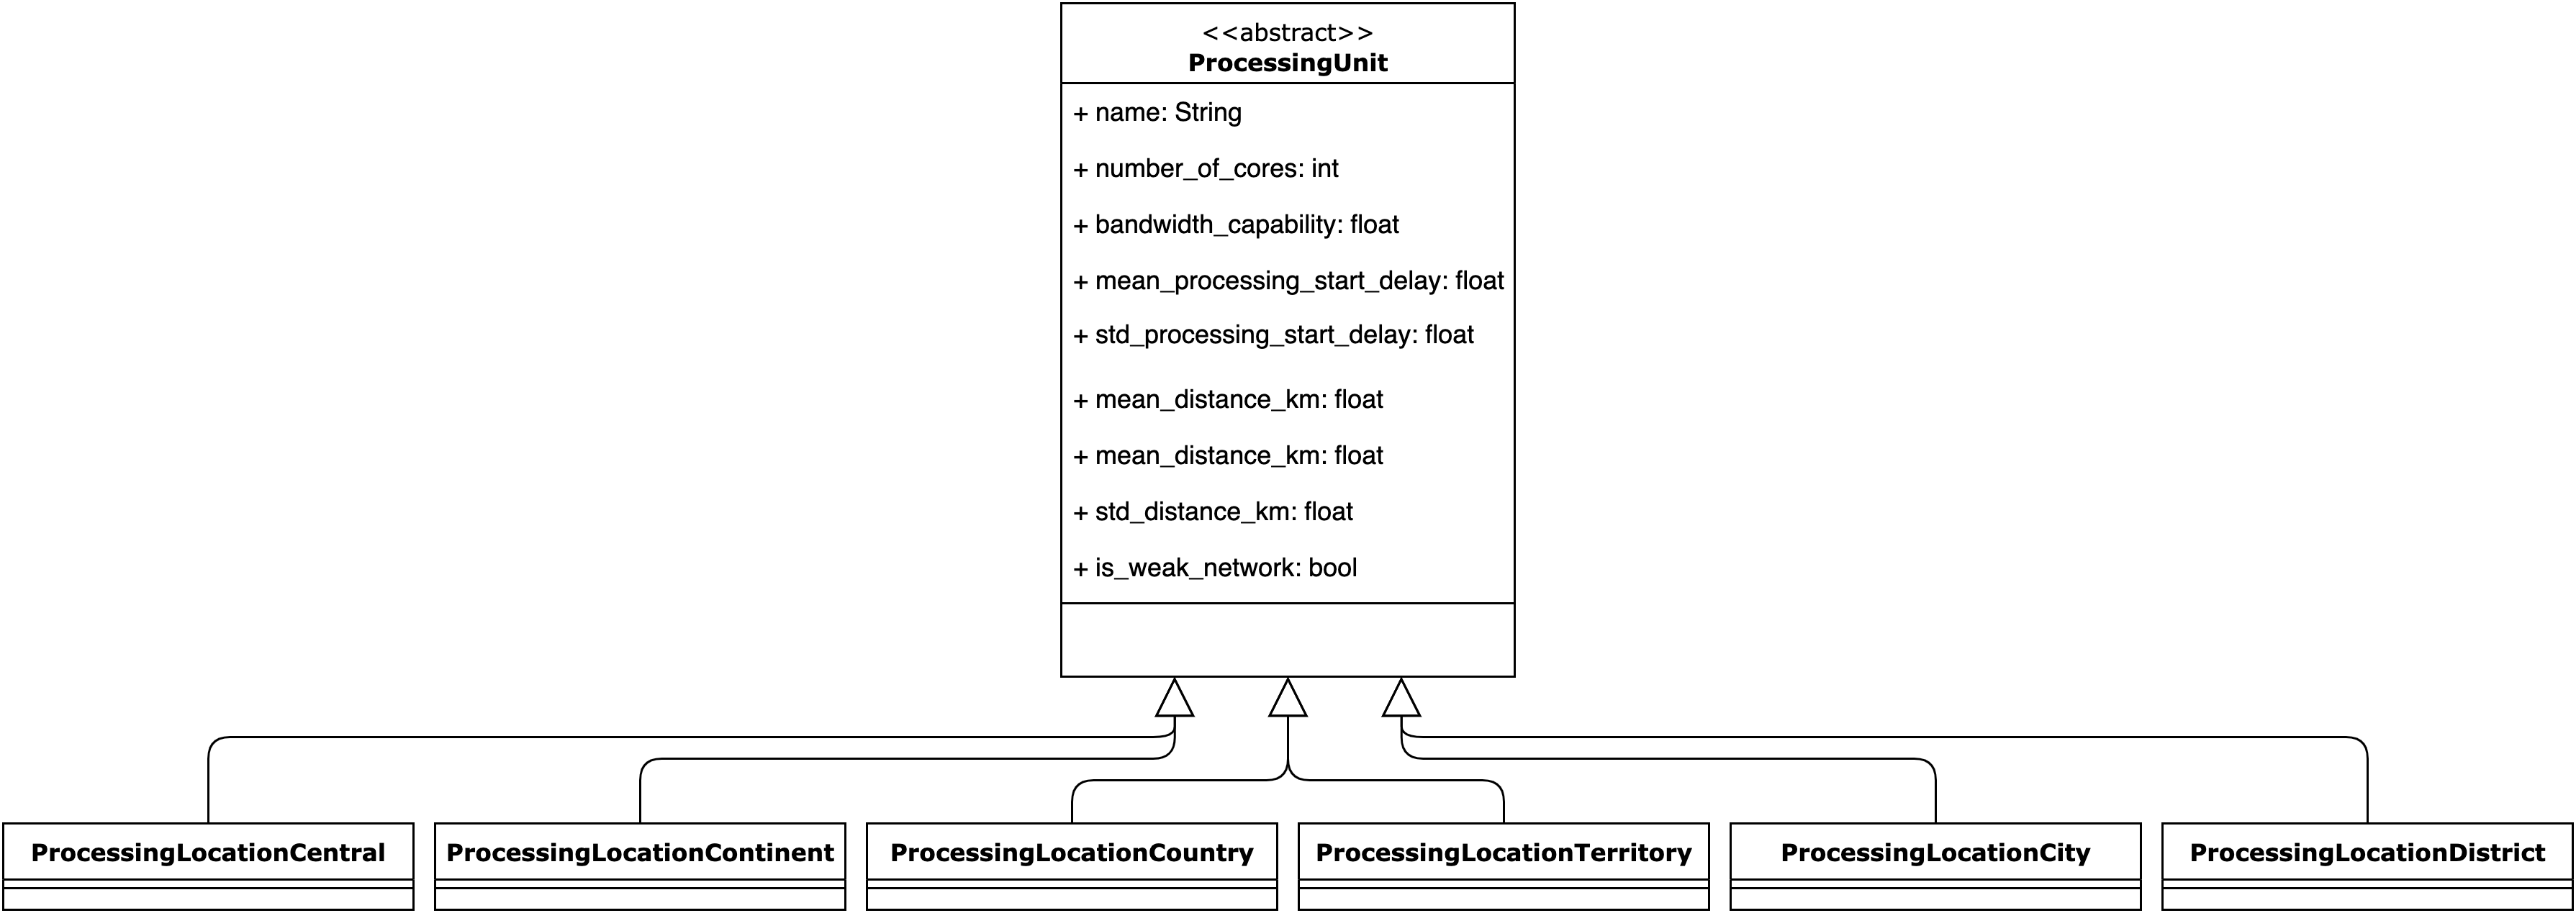
\includegraphics[width=0.99\linewidth]{Figures/Evaluation/processing-unit-realizations.png}
    \caption{Concrete realizations of the ProcessingUnit component.}
    \label{fig:processing-unit-realizations}
\end{figure}


\subsection{Matching the Abstractions to a Use Case}
To better narrow down the abstractions we can see in one of our use cases how these abstractions match a real scenario: in the traffic use case (TODO ref to use case chapter) the \inlinecode{DataProducerClient} represents the camera producing frames of the road. In our edge scenario the camera sends the frame to the lowest level in the hierarchy, which in our example architecture correspond to the "district" level (\inlinecode{ProcessingLocationDistrict}). While in the core-centric scenario the camera sends the frame to the central cloud (\inlinecode{ProcessingLocationCentral}).

The action of sending the frame is simulated using the \inlinecode{Transmission} component. The frame is then processed by applying an image recognition algorithm, an algorithm which is simulated as a data processing by the receiving \inlinecode{ProcessingUnit}.

In the core-centric scenario the output data is ready when finished processing. While in our edge scenario the ouput data is sent to the specified aggregating \inlinecode{ProcessingUnit} which needs to save the data. The communication is again simulated using the \inlinecode{Transmission} component, while the saving of data is simulated as a small processing of data in the aggregating \inlinecode{ProcessingUnit}.

A client can then need to know the traffic in a specific area. This is simulated using the \inlinecode{DataReaderClient} component which can send a read request message, sent using the \inlinecode{Transmission} component and processed by the receiving \inlinecode{ProcessingUnit}.


\subsection{Simulation Setting}
\label{section:simulation_setting}
Since the setting is similar in the various experiments, we present in the tables below the default values of the variables used in the experiments. The actual value will be extracted case by case from a normal distribution truncated to the left at zero. If the standard deviation is zero the value is actually a constant. Unless specified otherwise the values specified here are the ones used in the experiments.

\begin{table}[H]
\centering
\begin{tabular}{|c|c|l|}
\rowcolor{bluepoli!40} % comment this line to remove the color
\hline
\textbf{Variable}       & \textbf{Mean}   & \textbf{Standard deviation}    \\ \hline \hline
Number of clients       & 2000            & 0                              \\ \hline
Time between requests   & 10s             & 3s                             \\ \hline
Message size            & 423KB           & 150KB                          \\ \hline
\end{tabular}
\caption{Default values for variables of DataProducerClient}
\label{tab:default_setting_data_producer}
\end{table}

\begin{table}[H]
\centering
\begin{tabular}{|c|c|l|}
\rowcolor{bluepoli!40} % comment this line to remove the color
\hline
\textbf{Variable}       & \textbf{Mean}   & \textbf{Standard deviation}   \\ \hline \hline
Number of clients       & 2000            & 0                             \\ \hline
Time between requests   & 5s              & 2s                            \\ \hline
Message size            & 10KB            & 1KB                           \\ \hline
\end{tabular}
\caption{Default values for variables of DataReaderClient}
\label{tab:default_setting_data_reader}
\end{table}

\begin{table}[H]
\centering
\begin{tabular}{|c|c|l|}
\rowcolor{bluepoli!40} % comment this line to remove the color
\hline
\textbf{Variable}      & \textbf{Mean}   & \textbf{Standard deviation}   \\ \hline \hline
Weak network delay     & 12ms            & 8ms                           \\ \hline
Robust network delay   & 3ms             & 1ms                           \\ \hline
\end{tabular}
\caption{Default values for variables of Transmission}
\label{tab:default_setting_transmission}
\end{table}

\begin{table}[H]
\centering
\begin{tabular}{|c|c|l|}
\rowcolor{bluepoli!40} % comment this line to remove the color
\hline
\textbf{Variable}               & \textbf{Mean}   & \textbf{Standard deviation}   \\ \hline \hline
Number of districts             & 1000            & 0                             \\ \hline
Distance client-district        & 20km            & 8km                           \\ \hline
Number of cores per district    & 2               & 0                             \\ \hline
Processing bandwidth per core   & 10MB/s          & 0                             \\ \hline
Processing start delay          & 5ms             & 2ms                           \\ \hline
\end{tabular}
\caption{Default values for variables of ProcessingLocationDistrict}
\label{tab:default_setting_district}
\end{table}

\begin{table}[H]
\centering
\begin{tabular}{|c|c|l|}
\rowcolor{bluepoli!40} % comment this line to remove the color
\hline
\textbf{Variable}               & \textbf{Mean}   & \textbf{Standard deviation}   \\ \hline \hline
Number of cities                & 400             & 0                             \\ \hline
Distance client-city            & 60km            & 15km                          \\ \hline
Distance district-city          & 50km            & 15km                          \\ \hline
Number of cores per city        & 2               & 0                             \\ \hline
Processing bandwidth per core   & 10MB/s          & 0                             \\ \hline
Processing start delay          & 5ms             & 2ms                           \\ \hline
\end{tabular}
\caption{Default values for variables of ProcessingLocationCity}
\label{tab:default_setting_city}
\end{table}

\begin{table}[H]
\centering
\begin{tabular}{|c|c|l|}
\rowcolor{bluepoli!40} % comment this line to remove the color
\hline
\textbf{Variable}               & \textbf{Mean}   & \textbf{Standard deviation}   \\ \hline \hline
Number of territories           & 200             & 0                             \\ \hline
Distance client-territory       & 300km           & 100km                         \\ \hline
Distance district-territory     & 290km           & 100km                         \\ \hline
Number of cores per district    & 4               & 0                             \\ \hline
Processing bandwidth per core   & 15MB/s          & 0                             \\ \hline
Processing start delay          & 4ms             & 1ms                           \\ \hline
\end{tabular}
\caption{Default values for variables of ProcessingLocationTerritory}
\label{tab:default_setting_territory}
\end{table}

\begin{table}[H]
\centering
\begin{tabular}{|c|c|l|}
\rowcolor{bluepoli!40} % comment this line to remove the color
\hline
\textbf{Variable}               & \textbf{Mean}   & \textbf{Standard deviation}   \\ \hline \hline
Number of countries             & 80              & 0                             \\ \hline
Distance client-country         & 700km           & 300km                         \\ \hline
Distance district-country       & 690km           & 300km                         \\ \hline
Number of cores per country     & 4               & 0                             \\ \hline
Processing bandwidth per core   & 15MB/s          & 0                             \\ \hline
Processing start delay          & 4ms             & 1ms                           \\ \hline
\end{tabular}
\caption{Default values for variables of ProcessingLocationCountry}
\label{tab:default_setting_country}
\end{table}

\begin{table}[H]
\centering
\begin{tabular}{|c|c|l|}
\rowcolor{bluepoli!40} % comment this line to remove the color
\hline
\textbf{Variable}               & \textbf{Mean}   & \textbf{Standard deviation}   \\ \hline \hline
Number of continents            & 7               & 0                             \\ \hline
Distance client-continent       & 1500km          & 500km                         \\ \hline
Distance district-continent     & 1490km          & 500km                         \\ \hline
Number of cores per continent   & 1000            & 0                             \\ \hline
Processing bandwidth per core   & 20MB/s          & 0                             \\ \hline
Processing start delay          & 4ms             & 1ms                           \\ \hline
\end{tabular}
\caption{Default values for variables of ProcessingLocationContinent}
\label{tab:default_setting_continent}
\end{table}

\begin{table}[H]
\centering
\begin{tabular}{|c|c|l|}
\rowcolor{bluepoli!40} % comment this line to remove the color
\hline
\textbf{Variable}           & \textbf{Mean}   & \textbf{Standard deviation}   \\ \hline \hline
Distance client-central     & 5000km          & 2000km                        \\ \hline
Distance district-central   & 4990km          & 2000km                        \\ \hline
Number of cores             & 1000            & 0                             \\ \hline
Processing bandwidth        & 20MB/s          & 0                             \\ \hline
Processing start delay      & 4ms             & 1ms                           \\ \hline
\end{tabular}
\caption{Default values for variables of ProcessingLocationCentral}
\label{tab:default_setting_central}
\end{table}


\subsection{Results}
In each experiment we ran our SimPy simulation and let thousands of clients connect to the thousands of cloudlets and data centers, we collected data about latencies, distances and traffic and now we show in this section the results.
By having many variables extracted from the truncated normal distributions, we are effectively running random experiments where it makes sense to show a confidence interval calculated on the list of samples obtained. But collecting numerous samples is easy in a simulation, in fact we obtained in all the experiments a really tight 95\% confidence interval that cannot even be seen on the plot.


\subsubsection{Write by level}
In this experiment we suppose that the developer wants a single geographical aggregation, this means that we are simulating as if we were using our framework with the \inlinecode{saveAlsoInIntermediateLevels} set to \inlinecode{false}.
The clients send their data to the bottom level of the hierarchy (\inlinecode{ProcessingLocationDistrict} in case of the edge approach, \inlinecode{ProcessingLocationCentral} in case of the cloud approach). The data is then processed and, in the case of the edge approach, forwarded to the \inlinecode{referringArea} that aggregates the data.

\begin{figure}[H]
    \centering
    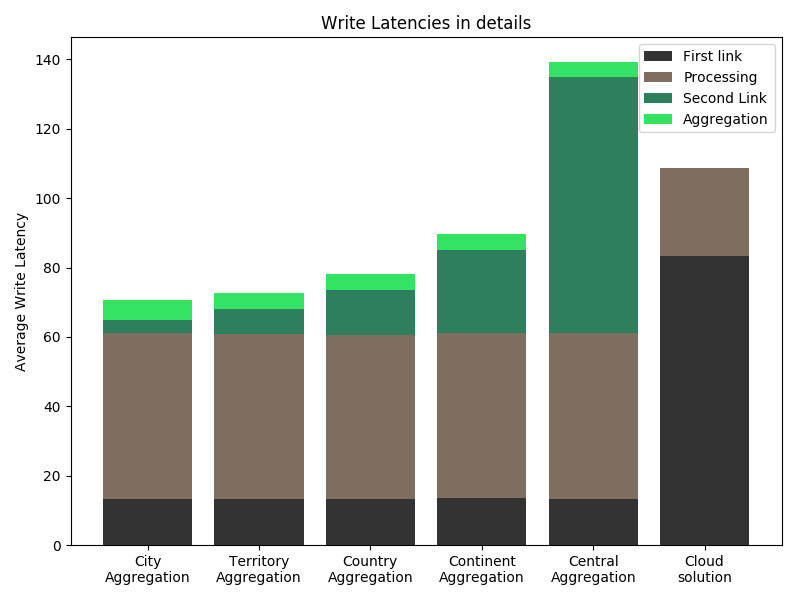
\includegraphics[width=0.86\linewidth]{Figures/Evaluation/write-by-latency2.png}
    \caption{Details on the average write latency compared between various aggregation in the edge setup and compared to the cloud setup.}
    \label{fig:write-by-latency2}
\end{figure}

In Figure \ref{fig:write-by-latency2} we can see the average write latency for each setup. For the edge approach we show the result of five different setups with five different levels of aggregation (city, territory, country, continent, central).
This average write latency comes from four different operations:
\begin{itemize}
    \item First link latency: latency of the communication between the client and the receiving machine.
    \item Processing latency: latency that considers the wait time for a core to be free and the processing time for the data sent by the client. We can see in the plot that the processing time of the cloud solution is close to half of the processing time in the edge setups, this is due the fact that the core bandwidth of a core in \inlinecode{ProcessingLocationCentral} is supposed to be double the core bandwidth of a core in \inlinecode{ProcessingLocationDistrict}.
    \item Second link latency: latency of the communication between the receiving  \inlinecode{ProcessingUnit} and the aggregating \inlinecode{ProcessingUnit}. This latency is only present in the setups using the edge approach.
    \item Aggregation latency: time required by the aggregating \inlinecode{ProcessingUnit} to save the data received from the \inlinecode{ProcessingLocationDistrict}. This time is the sum of the wait time for a core to be free and the time to save the processed data.
\end{itemize}

This result shows that with the edge approach using any aggregation level we have a smaller average latency than the cloud solution thanks to a much smaller travel distance needed to reach the aggregating \inlinecode{ProcessingUnit}. The only exception is the central aggregation of the edge approach, which is expected since it has the same travel distance of the cloud solution, but by doing the processing on the lower level of the hierarchy we have a smaller processing power.

Using this same experiment we now analyze the huge improvements our edge approach gives to the traffic in the network.

\begin{figure}[H]
    \centering
    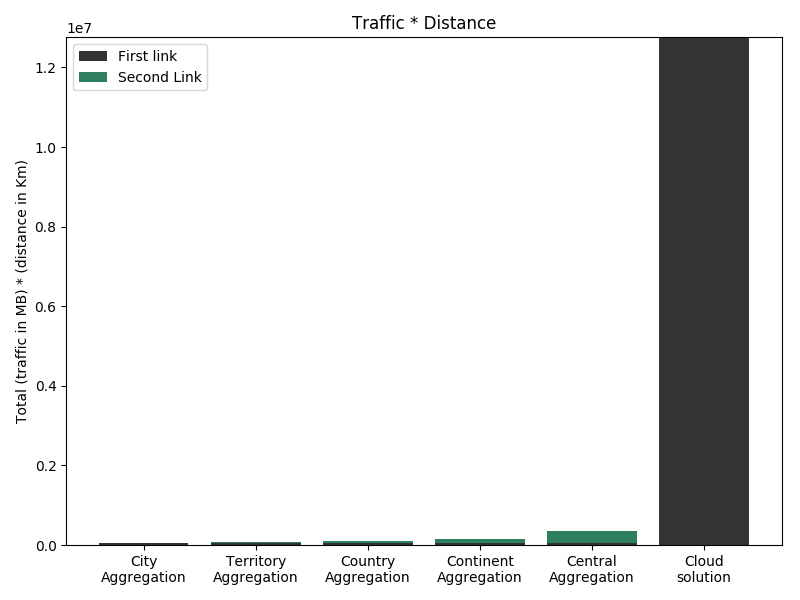
\includegraphics[width=0.86\linewidth]{Figures/Evaluation/write-by-traffic1.png}
    \caption{Traffic per distance generated in the network.}
    \label{fig:write-by-traffic1}
\end{figure}

In Figure \ref{fig:write-by-traffic1} we show the total traffic in megabytes multiplied by the distance travelled. This visualization is used to show that the cloud solution clogs the entire network, instead by processing the data near the client we obtain a huge saving in terms of bandwidth used in the network.

\begin{figure}[H]
    \centering
    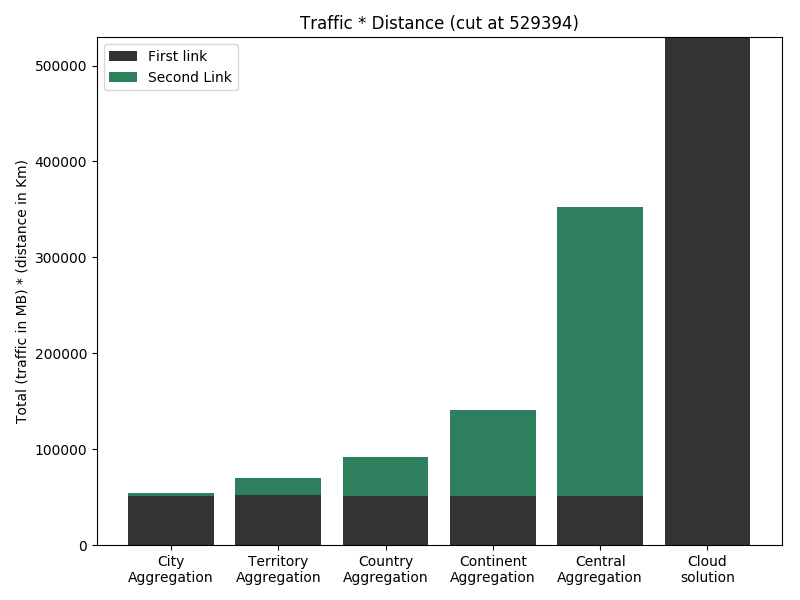
\includegraphics[width=0.86\linewidth]{Figures/Evaluation/write-by-traffic2.png}
    \caption{Traffic per distance generated in the network (cut at a lower traffic*distance value).}
    \label{fig:write-by-traffic2}
\end{figure}

In Figure \ref{fig:write-by-traffic2} we zoom on the values of the setups of the edge approach by cutting the plot at a lower traffic*distance value. We can see how the traffic*distance values in the first link for the edge approach are very much similar since in all five setups we have the same communication between the \inlinecode{DataProducerClient} and the \inlinecode{ProcessingLocationDistrict}. While for the second link we find an increase in the traffic*distance due to the fact that the distance increases between the \inlinecode{ProcessingLocationDistrict} and the aggregating \inlinecode{ProcessingUnit}.


\subsubsection{Write all levels}
In this experiment, for the edge approach, we suppose that the developer uses the boolean \inlinecode{saveAlsoInIntermediateLevels} set to \inlinecode{true} and sets the \inlinecode{referringAreaType} in our framework to the highest level of the hierarchy (central). Meaning that all writes made at the receiving  \inlinecode{ProcessingLocationDistrict} are forwarded to the upper levels. This setup is compared to the cloud setup in which data are sent to a central data center that can aggregate them by location.

Writes to upper levels happen in parallel, so we expect to have an average latency similar to the latency of the edge setup with central aggregation of the previous experiment. This is in fact what we obtain as can be seen in Figure \ref{fig:write-all-latency}. In terms of latency we are clearly in a case of disadvantage here since as it has been seen in the previous experiment that by doing a central aggregation, like the cloud approach does, we are not exploiting our edge approach to the max.

\begin{figure}[H]
    \centering
    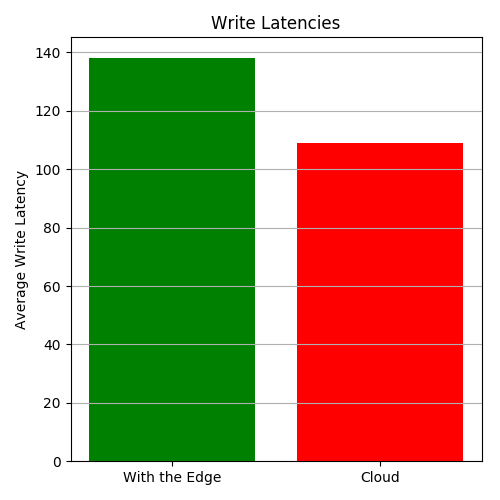
\includegraphics[width=0.75\linewidth]{Figures/Evaluation/write-all-latency.png}
    \caption{Average write latency of the single edge setup compared to the cloud setup.}
    \label{fig:write-all-latency}
\end{figure}

Many more messages are sent in parallel to the various aggregating \inlinecode{ProcessingUnit} so we expect the traffic*distance in the network to increase compared to the previous experiment. This is in fact true as can be seen in Figure \ref{fig:write-all-traffic1}, but still the cloud setup clogs the network 2000\% more than the edge setup.

\begin{figure}[H]
    \centering
    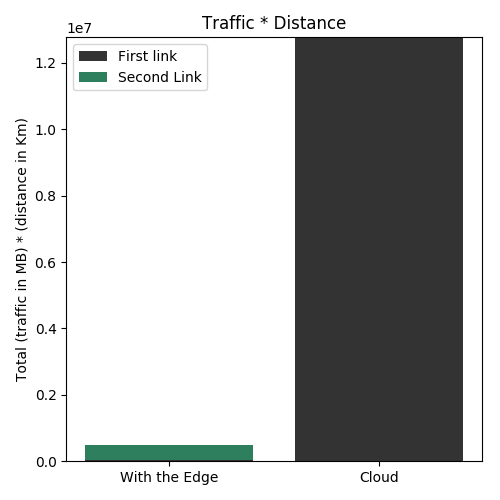
\includegraphics[width=0.75\linewidth]{Figures/Evaluation/write-all-traffic1.png}
    \caption{Traffic per distance generated in the network.}
    \label{fig:write-all-traffic1}
\end{figure}

We saw in this experiment that even in a disadvantage situation where our approach is used to aggregate the data in a central manner, which is not the intended use case, the increase in write latency is less than 27\%, but the improvement in terms of traffic sent in the network is tremendous.


\subsubsection{Write all levels, with cores performance as parameter}
As in the previous experiment we are working in a scenario where the developer imposes writes on all levels in the edge approach.

In our simulation we represented the performance of the cores as a processing bandwidth, so we specified how much megabytes a core can process in a second. In the previous experiments we used the default values reported in Section \ref{section:simulation_setting}, so we arbitrarily assumed that the \inlinecode{ProcessingLocationDistrict} and \inlinecode{ProcessingLocationCity} have 50\% of the performance of \inlinecode{ProcessingLocationCentral}. We now analyze the behaviour of the latency while slowly changing this percentage to show that the increase in write latency is not substantial.

\begin{figure}[H]
    \centering
    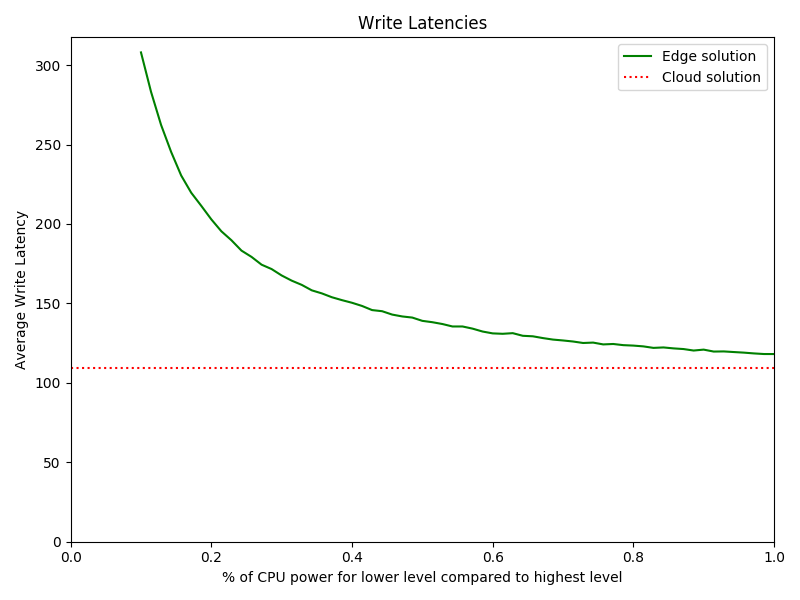
\includegraphics[width=0.86\linewidth]{Figures/Evaluation/write-all-cpu-latency.png}
    \caption{Average write latency of the edge solution as a function of the cores performance of lower levels}
    \label{fig:/write-all-cpu-latency}
\end{figure}

In Figure \ref{fig:/write-all-cpu-latency} it is shown the changing write latency of the edge solution due to the changing performance of the \inlinecode{ProcessingUnits} cores, compared to the constant latency of the cloud solution.

Note that the value 0.1 on the x-axis means that the performance of the core at the edge is 0.1 times (10\%) the performance of the core of cloud solution.

From 1.0 to 0.40 we have an almost linear increase, which is not substantial. Then down from 0.40 the cores can't keep up with the requests and start to put them in queue, creating an exponential increase in the latency.

So this experiment shows the following:
\begin{itemize}
    \item By having a lower performance in the \inlinecode{ProcessingUnits} at the edge the processing latency increase linearly, making the write latency also increase linearly;
    \item By having a lower performance in the \inlinecode{ProcessingUnits} at the edge it becomes easier to reach a limit where the cores can't keep up with the requests, creating an exponential increase in the write latency.
\end{itemize}


\subsubsection{Write all levels, with number of clients as parameter}
In this experiment we are again working in the scenario where the developer imposes writes on all levels while using the edge approach. But now we want to simulate, in this extreme setup, how our framework behaves when the number of clients rises without modifying other parameters.
We start from 1000 clients, rising up to 350'000 clients.

\begin{figure}[H]
    \centering
    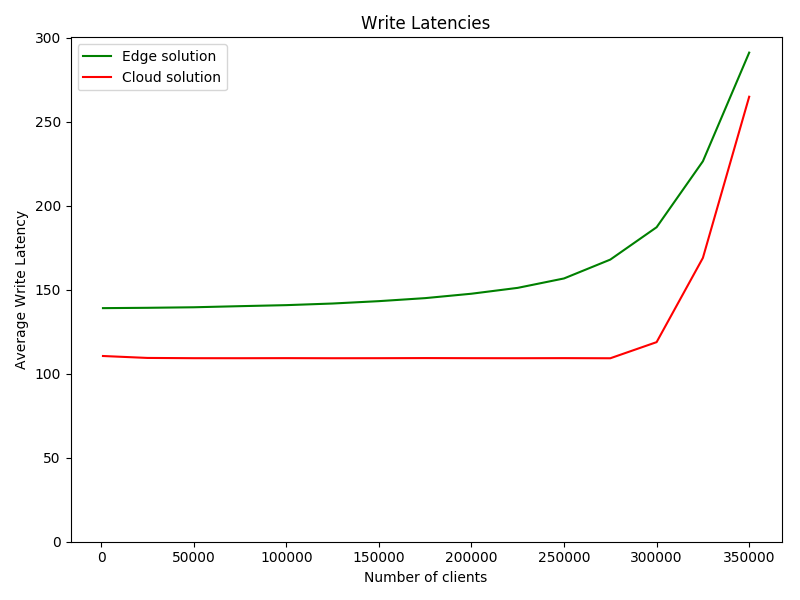
\includegraphics[width=0.86\linewidth]{Figures/Evaluation/write-all-clients-latency.png}
    \caption{Average write latency as a function of the number of clients}
    \label{fig:/write-all-clients-latency}
\end{figure}

As expected we see in Figure \ref{fig:/write-all-clients-latency} that, when the number of clients becomes too much to handle, both the cores at the edge and the cores in the cloud are overwhelmed and can't keep up with the requests causing the queues to grow indefinitely and consequently making the average latency grow.

We can also notice how the number of cores affects the latency: in the edge approach by having a low number of cores it's easier to be unlucky and having a momentary spike where the \inlinecode{ProcessingLocationDistrict} can't keep up with the requests, causing new requests to be queued for a short time. Basically by increasing the number of clients it become more probable to have a random spike in the requests, that a single \inlinecode{ProcessingLocationDistrict} cannot handle immediately since equipped with only 2 cores. This phenomenon causes a continuous increase in the average latency for the edge solution.
Instead in the cloud solution, to start to queue requests we have to first fill the 1000 cores, and for that to happen it needs many more clients.

It's important also to consider that in our simulation we are not modelling the access to the database: in a cloud scenario in which writes happen to a single instance of the database it can easily become a bottleneck if not replicated and handed correctly.

But again the improvements relative to the traffic generated in the network are immense. In Figure \ref{fig:/write-all-clients-traffic} we show the total traffic*distance as a function of the number of clients. Both the edge solution and cloud solution have a linear increase, but the coefficient of the increase in the cloud solution is evidently bigger than the one of the edge solution.

\begin{figure}[H]
    \centering
    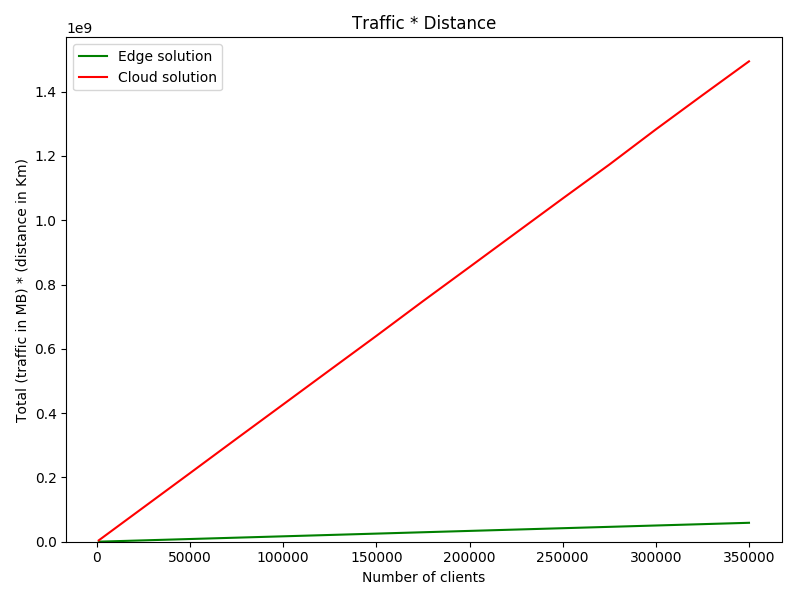
\includegraphics[width=0.86\linewidth]{Figures/Evaluation/write-all-clients-traffic.png}
    \caption{Total traffic*distance as a function of the number of clients}
    \label{fig:/write-all-clients-traffic}
\end{figure}

In this experiment we showed that our framework can keep up effectively with heavy load, with only minor random congestions at the lower levels of the hierarchy. But still provide immensely benefits in term of traffic through the network.


\subsubsection{Read by level}
We now start with a new type of experiment, focusing on the reads and not on the writes. We will immediately see the benefit on the latency since by having a geographical aggregation we can avoid to travel huge distances.
In practice in this experiment we have different setups in which every \inlinecode{DataReaderClients} in the setup communicates to a certain level of the hierarchy of the edge solution. While in the cloud solution they can only communicate to the central cloud.
In the figures reported below we can see, for each level of aggregation, the average latency and the average distance traveled, compared to the cloud solution.

\begin{figure}[H]
\begin{minipage}{0.49\textwidth}
\centering
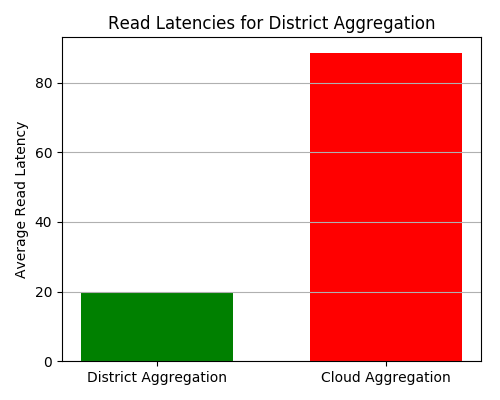
\includegraphics[width=1\linewidth]{Figures/Evaluation/read-by-latency-District-Aggregation.png}
\end{minipage}
\hfill
\begin{minipage}{0.49\textwidth}
\centering
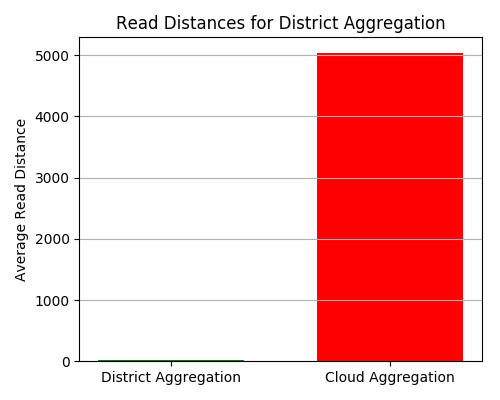
\includegraphics[width=1\linewidth]{Figures/Evaluation/read-by-distance-District-Aggregation.png}
\end{minipage}
\label{fig:read-by-district}
\caption{Average latency and average distance traveled for the district aggregation compared to a central aggregation}
\end{figure}

\begin{figure}[H]
\begin{minipage}{0.49\textwidth}
\centering
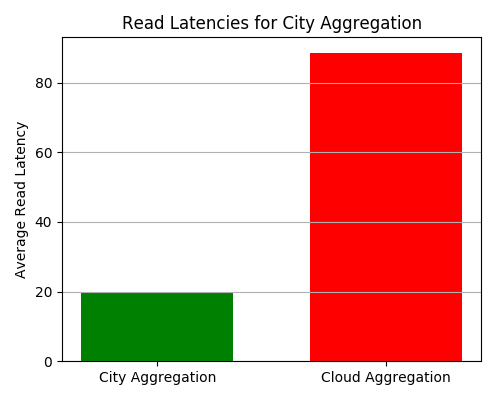
\includegraphics[width=1\linewidth]{Figures/Evaluation/read-by-latency-City-Aggregation.png}
\end{minipage}
\hfill
\begin{minipage}{0.49\textwidth}
\centering
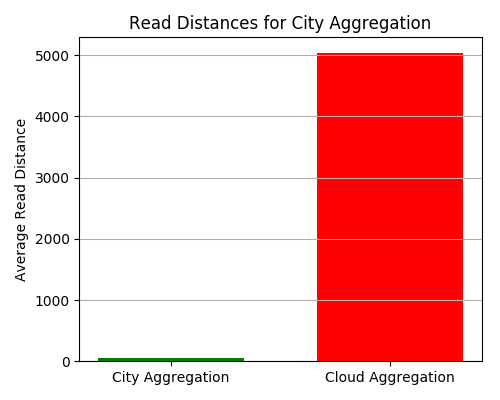
\includegraphics[width=1\linewidth]{Figures/Evaluation/read-by-distance-City-Aggregation.png}
\end{minipage}
\label{fig:read-by-city}
\caption{Average latency and average distance traveled for the city aggregation compared to a central aggregation}
\end{figure}

\begin{figure}[H]
\begin{minipage}{0.49\textwidth}
\centering
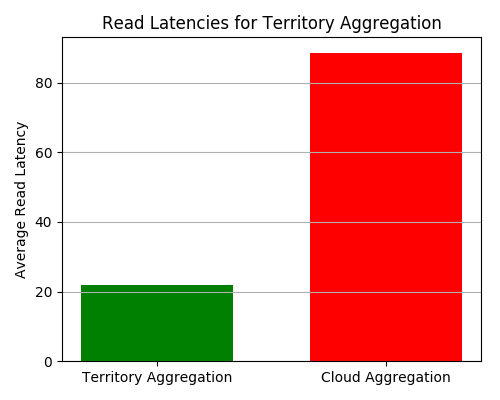
\includegraphics[width=1\linewidth]{Figures/Evaluation/read-by-latency-Territory-Aggregation.png}
\end{minipage}
\hfill
\begin{minipage}{0.49\textwidth}
\centering
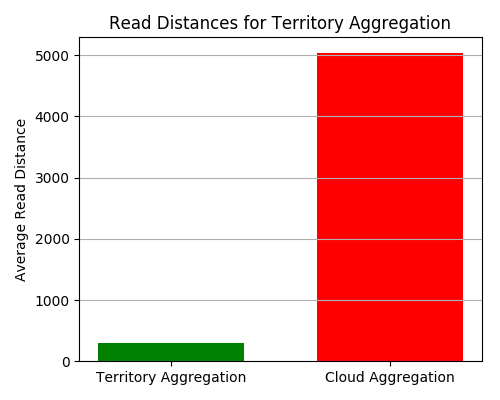
\includegraphics[width=1\linewidth]{Figures/Evaluation/read-by-distance-Territory-Aggregation.png}
\end{minipage}
\label{fig:read-by-territory}
\caption{Average latency and average distance traveled for the territory aggregation compared to a central aggregation}
\end{figure}

\begin{figure}[H]
\begin{minipage}{0.49\textwidth}
\centering
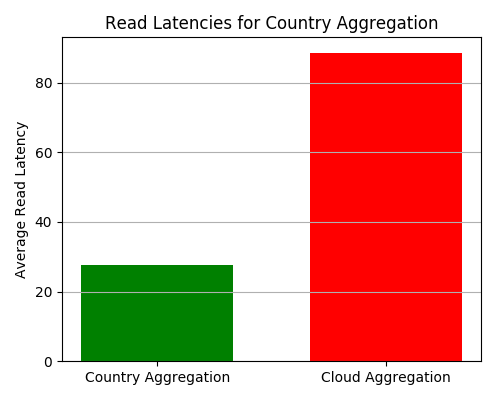
\includegraphics[width=1\linewidth]{Figures/Evaluation/read-by-latency-Country-Aggregation.png}
\end{minipage}
\hfill
\begin{minipage}{0.49\textwidth}
\centering
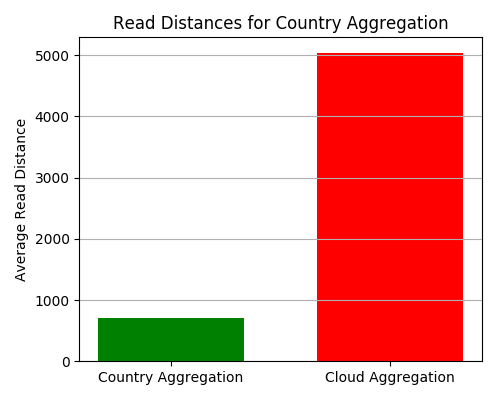
\includegraphics[width=1\linewidth]{Figures/Evaluation/read-by-distance-Country-Aggregation.png}
\end{minipage}
\label{fig:read-by-country}
\caption{Average latency and average distance traveled for the country aggregation compared to a central aggregation}
\end{figure}

\begin{figure}[H]
\begin{minipage}{0.49\textwidth}
\centering
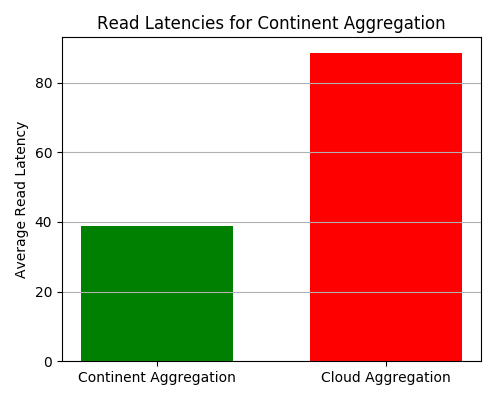
\includegraphics[width=1\linewidth]{Figures/Evaluation/read-by-latency-Continent-Aggregation.png}
\end{minipage}
\hfill
\begin{minipage}{0.49\textwidth}
\centering
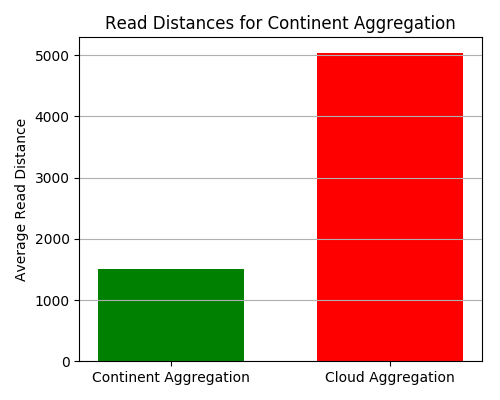
\includegraphics[width=1\linewidth]{Figures/Evaluation/read-by-distance-Continent-Aggregation.png}
\end{minipage}
\label{fig:read-by-continent}
\caption{Average latency and average distance traveled for the continent aggregation compared to a central aggregation}
\end{figure}

If we go up in the hierarchy to perform the aggregation we become more distant to the reading client, creating a bigger latency on average.

We can see also how the average latency is proportional to the average distance: when the distance increases, so does the latency due to the bigger travel distance.

If we compare the best scenario, in which the aggregation is performed at the lowest level, to the cloud solution we see that the cloud solution creates a latency 350\% bigger than the district (19.5 ms compared to 88.5 ms). 


\subsubsection{Read all levels}
This time we allow clients to perform the reads on every level, this means that to have the data available the writes must have happen with the \inlinecode{saveAlsoInIntermediateLevels} boolean set to \inlinecode{true}.
In the 51 setups that we ran we increased the probability of making a read on an upper level of the hierarchy. The first setup performs all the read requests at the district level, in the intermediate setup the clients perform the read requests with almost an equal probability to all levels, while the last setup performs all the read requests to the single central level.

\begin{figure}[H]
    \centering
    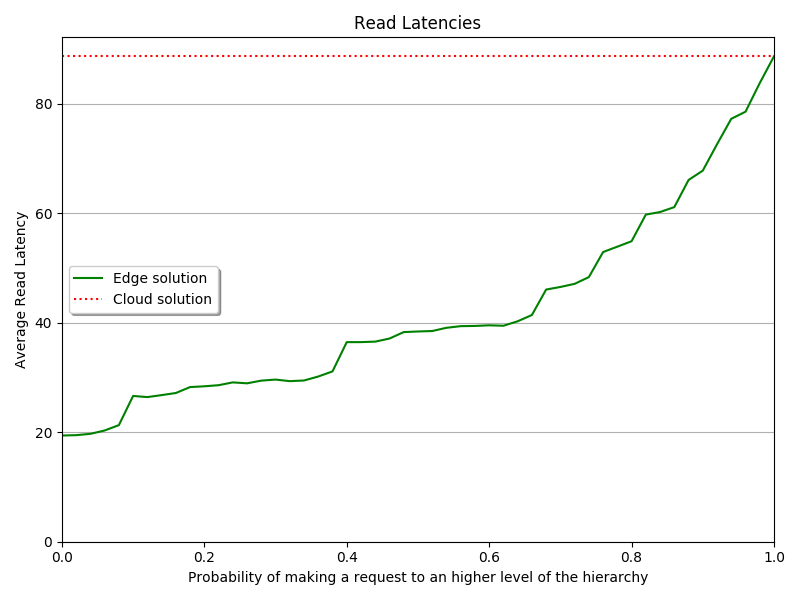
\includegraphics[width=0.86\linewidth]{Figures/Evaluation/read-all-latency.png}
    \caption{Average read latency as a function of the probability of making the read request to an higher level}
    \label{fig:/read-all-latency}
\end{figure}

\begin{figure}[H]
    \centering
    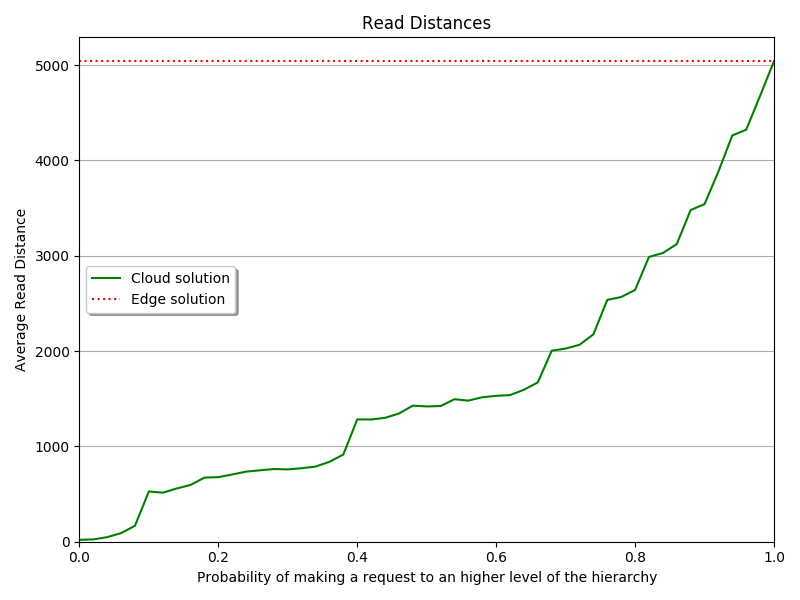
\includegraphics[width=0.86\linewidth]{Figures/Evaluation/read-all-distance.png}
     \caption{Average distance traveled for the request as a function of the probability of making the read request to an higher level}
    \label{fig:/read-all-distance}
\end{figure}

As expected we see a monotonic increase in the latency and a strict correlation between the average distance traveled and the average latency.

\subsubsection{Read district level, with cores performance as parameter}
In this experiment clients make read requests to the lowest level of the hierarchy, the district level, and we study the latency as a function of the cores performance of this level.
We arbitrarily assumed that the \inlinecode{ProcessingLocationDistrict} has 50\% of the performance of \inlinecode{ProcessingLocationCentral}, but now we slowly change this percentage to analyze the behaviour of the latency.

\begin{figure}[H]
    \centering
    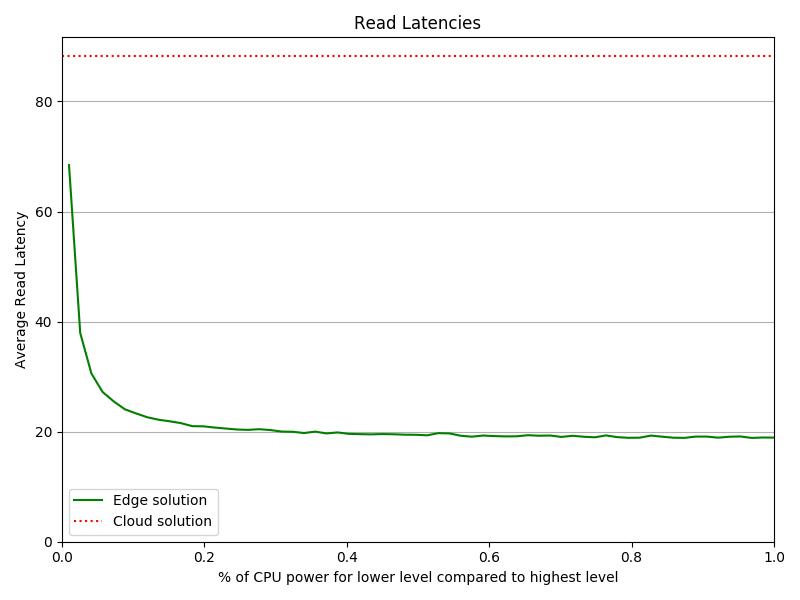
\includegraphics[width=0.86\linewidth]{Figures/Evaluation/read-district-cpu-latency.png}
    \caption{Average read latency of the edge solution as a function of the cores performance of lower levels}
    \label{fig:/read-district-cpu-latency}
\end{figure}

As can be seen in Figure \ref{fig:/read-district-cpu-latency}, the effects of slower cores start to affect the latency only when reaching very low percentages i.e., 10\%, and still even at 1\% of the performance the latency is smaller than the one of the cloud solution. This is because a read request is a fast operation and is not a processing intensive task, so the cores can manage the load comfortably.

\subsubsection{Read district level, with number of clients as parameter}
As a last experiment we see how the framework performs in the simulations with a varying number of clients (and consequently a varying load).
Similarly here read requests are made to the lowest level of the hierarchy, the district level.

\begin{figure}[H]
    \centering
    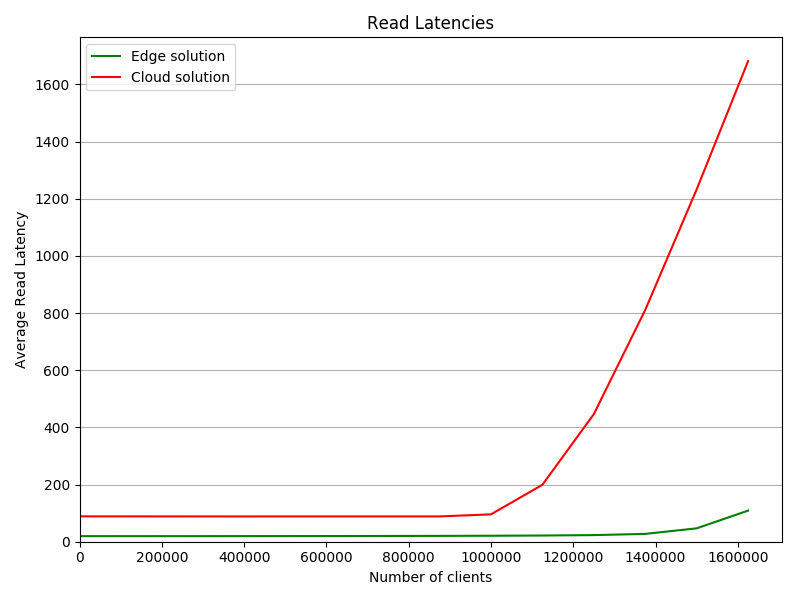
\includegraphics[width=0.86\linewidth]{Figures/Evaluation/read-district-clients-latency.png}
    \caption{Average read latency of the edge solution as a function of the number of clients}
    \label{fig:/read-district-clients-latency}
\end{figure}

The read operation is a fast operation that does not require heavy processing, this allows both the cloud solution and the edge solution to fulfill a million of requests in a small amount of time before starting to not keep up with the load.

\subsection{Summing Up}
Thanks to the simulation and by performing the various experiments we showed that by using our framework we get immense benefits in terms of reduced traffic in the network while allowing faster reads when the data aggregation needed is not central.
In a case where a central aggregation is still needed we showed that the write requests suffer an increase in latency, but the increase is not substantial.

We also noticed how our edge solution can be affected by random spikes in the requests due to the small number of cores and resources in the lowest level of the hierarchy, so there is a clear room for improvements on this matter, but still the increase in latency is not drastic.


\chapter{Conclusions and future developments}
\label{ch:conclusions}
TODO


\section{Conclusions}
TODO


\section{Future Works}
TODO


\iffalse
In this chapter, you present the conclusions of your thesis and a couple of possible future works to extend your results. First of all, you should briefly repeat the problem you addressed in the thesis. Then, you report your achievements and how they improve the state of the art.

\section{Conclusions}
In this thesis, we analyzed the problem of ... . We proposed a new approach that ... . We tested this method on ... . Reported results show that our proposal outperforms the state of the art method.

\section{Future works}
There are several appealing paths for future works. A possible extension could be to ... .
\fi

\cleardoublepage

%-------------------------------------------------------------------------
%	APPENDICES
%-------------------------------------------------------------------------

\addtocontents{toc}{\vspace{2em}} % Add a gap in the Contents, for aesthetics
\appendix
\chapter{Appendix}

The resulting artifacts of our research have been released as open-source software \cite{thesis-github}. Here we present a concise guide on how to run and use these artifacts.

Note that this guide is not meant to be universal, and instead shows the steps we performed to run the system in our specific setup.

\section{Running the Prototype}
For running the prototype we used the \textit{faas} flavour of \textit{OpenFaas}, which runs on top of \textit{Kubernetes}. If \textit{faasd}, the lighter version of \textit{OpenFaas}, is needed, then a slightly different setup would be necessary.


\subsection{Prerequisites}
The following applications and Command Line Interface programs are needed to setup the framework:
\begin{itemize}
    \item \textbf{arkade}: \textit{arkade} provides a portable marketplace for downloading popular devops CLIs and installing helm charts;
    \\It can be installed with \inlinecode{curl -sLS https://get.arkade.dev | sudo sh};
    \\More info at this link \href{https://github.com/alexellis/arkade}{github.com/alexellis/arkade}
    
    \item \textbf{faas-cli}: the Command Line Interface of \textit{OpenFaas};
    \\It can be installed with \inlinecode{arkade get faas-cli};
    
    \item \textbf{helm}: the \textit{Kubernetes} package manager;
    \\It can be installed with \inlinecode{arkade get helm};
    
    \item \textbf{minikube}: a local \textit{Kubernetes} engine;
    \\On our setup running macOS Big Sur with a x86-64 CPU it was installed with \inlinecode{brew install minikube};
    \\More info at this link \href{https://minikube.sigs.k8s.io/docs/start/}{minikube.sigs.k8s.io/docs/start/}
\end{itemize}


\subsection{Kubernetes Setup}
To run \textit{Kubernetes} we used \textit{minikube}, a software which allows to easily create a Virtual Machine environment equipped with \textit{Kubernetes}. Note that in a production environment \textit{minikube} is not recommended, but in our emulation it was perfect to run multiple nodes that emulate the nodes in an edge network.

The following are the commands we used to start the Virtual Machines (note that as virtualization software connected to \textit{minikube} we used \textit{Parallels Desktop}):
\begin{lstlisting}[language=bash]
minikube delete --all  # Delete previous VMs

minikube config set driver parallels  # Set Parallels as virtualization software

minikube config set cpus 2  # Set 2 CPUs per VM

minikube config set memory 2048  # Set 2048MB of RAM per VM

minikube start --profile p1  # Start a new VM with name p1

minikube start --profile p2  # Start a new VM with name p2

minikube ip --profile p1  #  Get IP address of p1

minikube ip --profile p2  #  Get IP address of p2

kubectl config get-contexts  #  Print Kubernetes contexts (should show two Kubernetes machines, p1 and p2)

kubectl config use-context p1  #  Use p1 for the next commands

kubectl get po -A  # List all pods running on Kubernetes
\end{lstlisting}

At the end of these commands the results are, in this case, the creation of two empty VMs running \textit{Kubernetes}, without any external software installed on it.
Now the goal is to install the framework we developed on top of these \textit{Kubernetes} installations.

Three steps are still needed:
\begin{itemize}
    \item Install the \textit{faas} flavour of \textit{OpenFaas} on top of \textit{Kubernetes};
    \item Install \textit{Redis} on top of Kubernetes;
    \item Deploy on \textit{OpenFaas} the function we developed that allows locations to receive forwarded write actions.
\end{itemize}


\subsection{OpenFaas Setup}
On each \textit{Kubernetes} environment it is needed to install \textit{OpenFaas}. The installation can be performed in the following way:
\begin{lstlisting}[language=bash]
# Use p1 for the next commands (should be changed for every VM)
kubectl config use-context p1

# Apply OpenFaas configuration
kubectl apply -f https://raw.githubusercontent.com/openfaas/faas-netes/master/namespaces.yml

# Write OpenFaas password in a secret
kubectl -n openfaas create secret generic basic-auth --from-literal=basic-auth-user=admin --from-literal=basic-auth-password="customOpenFaasPassword"  

# Install OpenFaas
helm upgrade openfaas --install openfaas/openfaas --namespace openfaas --set functionNamespace=openfaas-fn --set basic_auth=true

# Install the cron addon
helm upgrade --install cron-connector openfaas/cron-connector --namespace openfaas

# Login to OpenFaas running on machine p1 that we have just installed
echo "customOpenFaasPassword" | faas-cli login -u admin --password-stdin --gateway http://$(minikube ip --profile p1):31112
\end{lstlisting}
At the end of this step we have the \textit{faas} flavour of \textit{OpenFaas} installed on every node.


\subsection{Redis Setup}
On each \textit{Kubernetes} environment it is needed to install \textit{Redis}. The installation can be performed in the following way:
\begin{lstlisting}[language=bash]
# Use p1 for the next commands (should be changed for every VM)
kubectl config use-context p1

# Install Redis
helm install my-openfaas-redis bitnami/redis --namespace openfaas-fn --set auth.password="customRedisPassword" --set master.persistence.enabled=false
\end{lstlisting}
At the end of this step we have a Redis instance installed on every node on top of \textit{Kubernetes}.
Now we can put all the IP addresses of the machines in the JSON of the infrastructure.
\\The IP addresses can be obtained, as seen, with \inlinecode{minikube ip --profile p1}.


\subsection{The Receiver Function}
After the infrastructure JSON file is ready we can deploy the function "edge-db-data-receiver" which allows locations to receive forwarded write actions.
\begin{lstlisting}[language=bash]
# Move in the directory where the "edge-db-data-receiver" function is stored
cd ./framework/functions-main/

# Build and publish the "edge-db-data-receiver" function on a Docker Registry
faas-cli publish --filter edge-db-data-receiver --platforms linux/arm/v7,linux/amd64

# Deploy the function on every level, except the lowest level
deployer deploy edge-db-data-receiver infrastructure.json --inEvery city
deployer deploy edge-db-data-receiver infrastructure.json --inEvery country
deployer deploy edge-db-data-receiver infrastructure.json --inEvery continent
\end{lstlisting}
At the end of this step the framework is ready to receive custom functions, that can be created by the developer as seen in Chapter \ref{ch:prototype}. 


\subsection{Deploying Custom Function}
To deploy new custom functions it is simply needed to perform the following commands:
\begin{lstlisting}[language=bash]
# Move in the directory where the "stack.yml" file is defined
cd ./framework/functions-main/

# Build and publish the function on a Docker Registry
faas-cli publish --filter my-function-name --platforms linux/arm/v7,linux/amd64

# Deploy the function
deployer deploy my-function-name infrastructure.json --inEvery district --inAreas italy paris --exceptIn milan
\end{lstlisting}


\section{Debugging the Prototype}

\subsection{Debugging Custom Functions}
The following commands can be used to print the logs of a function:
\begin{lstlisting}[language=bash]
# Select which node to debug
kubectl config use-context p1

# Print the logs of the function running on that node
kubectl logs -n openfaas-fn deploy/my-function-name -f
\end{lstlisting}
Or alternatively the \textit{faas-cli} can be used as follows:
\begin{lstlisting}[language=bash]
faas-cli logs my-function-name --gateway http://$(minikube ip --profile p1):31112
\end{lstlisting}


\subsection{Debugging the Framework}
To debug the framework itself or to understand why a function is having issues starting up, the following commands can be used:
\begin{lstlisting}[language=bash]
# Select which node to debug
kubectl config use-context p1

# List all pods and components running on Kubernetes
kubectl get po -A

# Print many info about a single component (in this example the gateway component)
kubectl describe -n openfaas deploy/gateway
kubectl logs -n openfaas deploy/gateway

# Print events happened in the openfaas namespace
kubectl get events -n openfaas --sort-by=.metadata.creationTimestamp
\end{lstlisting}


\section{Running the Simulation}
The Simulation is composed of many Phython files, one file for each scenario. To run a scenario it is simply possible to run the Python file with a Python IDE (e.g., PyCharm).

Note that a single configuration in some scenarios may simulate millions of machines and the simulation of such a huge number of machines requires an high utilization of RAM.
For example the scenario included in \inlinecode{simulation\_read\_district\_level\_clients\_ratio.py} can use up to 14 GB or RAM for the simulation.
If such usage of RAM becomes a problem, it is possible to make a modification to the trade-off between the speed of the execution of the simulation and the usage of RAM by modifying the following line:\\
\inlinecode{pool = multiprocessing.Pool(processes=4)}\\
and replacing the 4 with a lower number to use less RAM, while also using less parallelism for the simulation, resulting in a slower execution. In practice this number represents how many configurations of the scenario can be run in parallel on the given processes.




% INFORMAL ACKNOWLEDGEMENTS
%\chapter*{Acknowledgments}
TODO


\iffalse
Here you can insert optionally the acknowledgments for who had a significant importance for the accomplishment of this goal. These acknowledgments are less formal than the ones at the beginning of the thesis and are not listed in the table of contents.
\fi


\cleardoublepage

%-------------------------------------------------------------------------
%	BIBLIOGRAPHY
%-------------------------------------------------------------------------

\addtocontents{toc}{\vspace{2em}} % Add a gap in the Contents, for aesthetics
\bibliography{Thesis_bibliography} % The references information are stored in the file named "Thesis_bibliography.bib"

\end{document}
